\documentclass[conference]{IEEEtran}

\usepackage{amsmath,amssymb,amsfonts}
\usepackage{graphicx}
\usepackage{textcomp}
\usepackage{xcolor}
\usepackage{url}
\usepackage[hidelinks]{hyperref}
\usepackage{booktabs}
\usepackage{float}
\usepackage{listings}
\usepackage{subcaption}
\usepackage[newfloat]{minted}
\pagestyle{plain}

\setminted{
    fontsize=\scriptsize,
    breaklines=true,
    bgcolor=gray!8,
    frame=none,
    xleftmargin=6pt
}

\lstdefinestyle{code}{
    backgroundcolor=\color{gray!8},
    basicstyle=\ttfamily\scriptsize,
    keywordstyle=\color{green!45!black}\bfseries,
    commentstyle=\color{gray},
    stringstyle=\color{red!60!black},
    breaklines=true,
    breakatwhitespace=false,
    postbreak=\mbox{\textcolor{gray}{$\hookrightarrow$}\space},
    frame=none,
    numbers=none,
    showstringspaces=false,
    captionpos=b,
    columns=fullflexible,
    keepspaces=true,
    xleftmargin=8pt,
    framexleftmargin=8pt,
    aboveskip=6pt,
    belowskip=6pt
}
\lstset{style=code}

% Plain style for the file tree
\lstdefinestyle{plain}{
    backgroundcolor=\color{gray!8},
    basicstyle=\ttfamily\scriptsize,
    breaklines=true,
    frame=none,
    numbers=none,
    showstringspaces=false,
    xleftmargin=8pt,
    framexleftmargin=8pt,
    aboveskip=6pt,
    belowskip=6pt
}

\raggedbottom

\begin{document}

\title{ACIT4820: Assignment 2 \\[4pt] \normalsize \textit{Total words: }}

\author{
    \IEEEauthorblockN{Felix Boehm}
    \IEEEauthorblockA{OsloMet \\ feboe8099@oslomet.no}
     \and
    \IEEEauthorblockN{Thomas Heim}
    \IEEEauthorblockA{OsloMet \\ thhei7342@oslomet.no}
}

\maketitle

\section{Method}
For task 1, we decided to make macros for the wheel as there was a lot of repetition. We replaced both with one drive\_wheel macro that has the link and the joint and takes a prefix and a position, and then called it twice. We also made macros for the inertia tensors. We made inertial\_box, inertial\_cylinder and inertial\_sphere, that take a mass and the dimensions and make up the whole inertial block. The wheels benefited from using macros since this is the structure in the robot that repeats. This makes sure that we have the same dimensions for the back wheels. The inertia macros were useful as the three formulas are used across four links. This makes the code more modular, as we don't have to hardcode the numbers. 

Task 2: 


For Task 3, we set the lidar laser first to 360 degrees because it scanned more, but we later changed it to 640 samples over plus-minus 80 degrees that the Gazebo documentation uses, so that our configurations matched what the assignment pointed to. For the radar itself, we added a cylindrical lidar\_link on top of the chassis with a fixed joint. We got the joint height from half the chassis height plus half the sensor height, rather than hardcoding it. We did this as this is more modular, in case we want to change the dimensions of e.g. the chassis in the future.

Task 4: 



\section{Results}
\subsection*{Task 1: Modularising with Xacro}

The description is split into five files. Only my\_robot.urdf.xacro can be
expanded on its own, since it includes the others in order. The remaining four
are fragments that use properties defined in parameters.xacro.

\begin{listing}[H]
\begin{minted}{text}
urdf/
├── my_robot.urdf.xacro   top level, includes only
├── parameters.xacro      dimensions, materials, macros
├── my_robot_core.xacro   links and joints
├── gazebo_control.xacro  friction and plugins
└── lidar.xacro           LiDAR link and sensor
\end{minted}
\caption{The five files making up the robot description.}
\label{lst:tree}
\end{listing}

\begin{figure}[H]
    \centering
    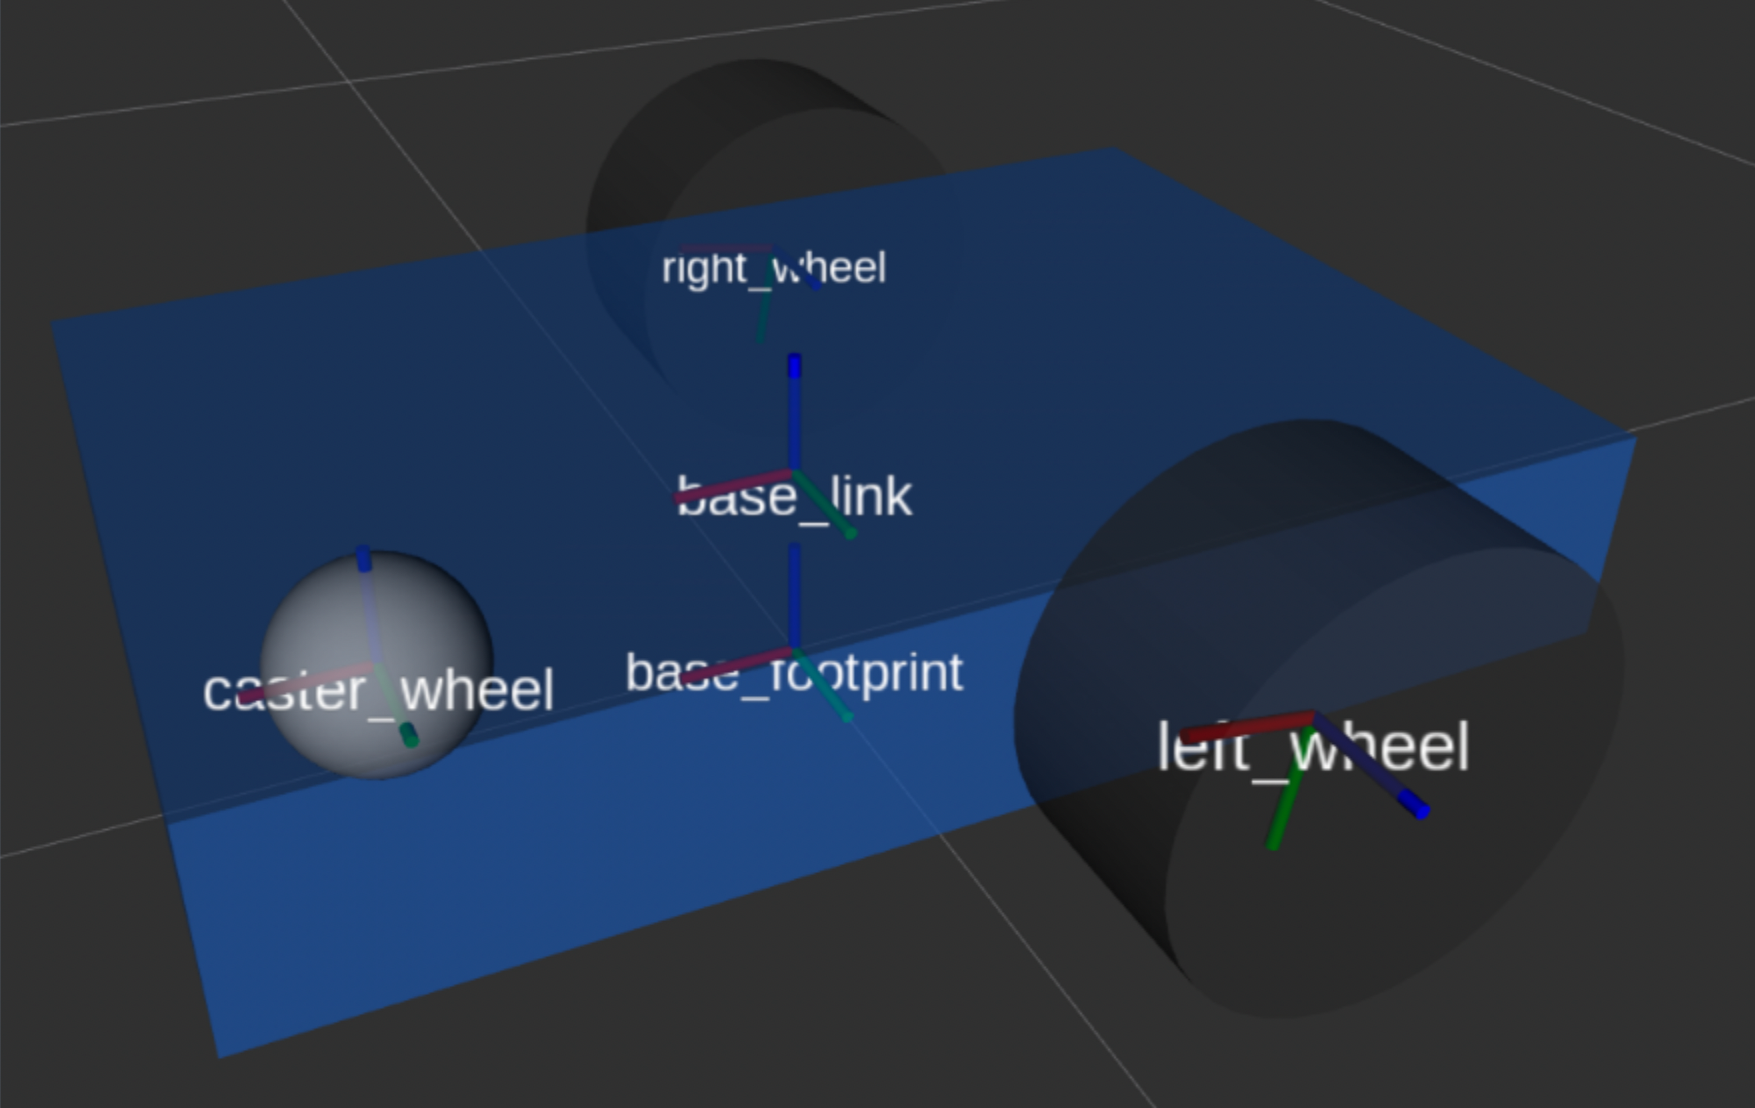
\includegraphics[width=\columnwidth]{fig/Task1/Task1Fig.png}
    \caption{The robot in RViz after the conversion to Xacro, unchanged from
             Assignment 1.}
    \label{fig:t1_rviz}
\end{figure}

\begin{figure}[H]
    \centering
    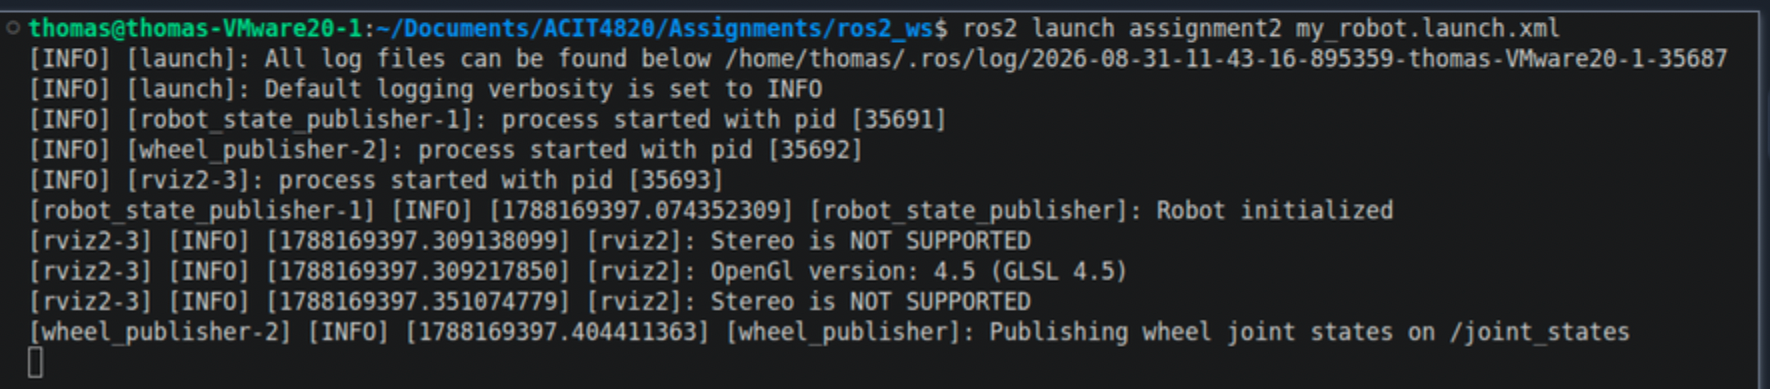
\includegraphics[width=\columnwidth]{fig/Task1/Task1Terminal.png}
    \caption{Terminal output from launching the Xacro based description.}
    \label{fig:t1_terminal}
\end{figure}

\subsection*{Task 2: World, physics and teleoperation}

The differential drive plugin reads the wheel separation and radius from the
same properties the wheels are built from, so the controller and the geometry
cannot disagree. The two frame settings are needed because Gazebo otherwise
names its frames after the model, which RViz cannot join to the rest of the
transform tree.

\begin{listing}[H]
\begin{minted}{xml}
<plugin filename="gz-sim-diff-drive-system"
        name="gz::sim::systems::DiffDrive">
  <left_joint>left_wheel_joint</left_joint>
  <right_joint>right_wheel_joint</right_joint>
  <wheel_separation>${wheel_separation}</wheel_separation>
  <wheel_radius>${wheel_radius}</wheel_radius>
  <odom_publish_frequency>50</odom_publish_frequency>
  <topic>cmd_vel</topic>
  <frame_id>odom</frame_id>
  <child_frame_id>base_footprint</child_frame_id>
</plugin>
\end{minted}
\caption{The differential drive plugin, from gazebo\_control.xacro.}
\label{lst:diffdrive}
\end{listing}

Each bridge entry names the topic and message type on both sides and the
direction it flows. Two of our six entries are shown; cmd\_vel is the only one
going from ROS into Gazebo, the rest carry simulation output back out.

\begin{listing}[H]
\begin{minted}{yaml}
- ros_topic_name: "cmd_vel"
  gz_topic_name: "cmd_vel"
  ros_type_name: "geometry_msgs/msg/Twist"
  gz_type_name: "gz.msgs.Twist"
  direction: ROS_TO_GZ

- ros_topic_name: "scan"
  gz_topic_name: "scan"
  ros_type_name: "sensor_msgs/msg/LaserScan"
  gz_type_name: "gz.msgs.LaserScan"
  direction: GZ_TO_ROS
\end{minted}
\caption{Two entries from config/gz\_bridge.yaml.}
\label{lst:bridge}
\end{listing}

\begin{figure}[H]
    \centering
    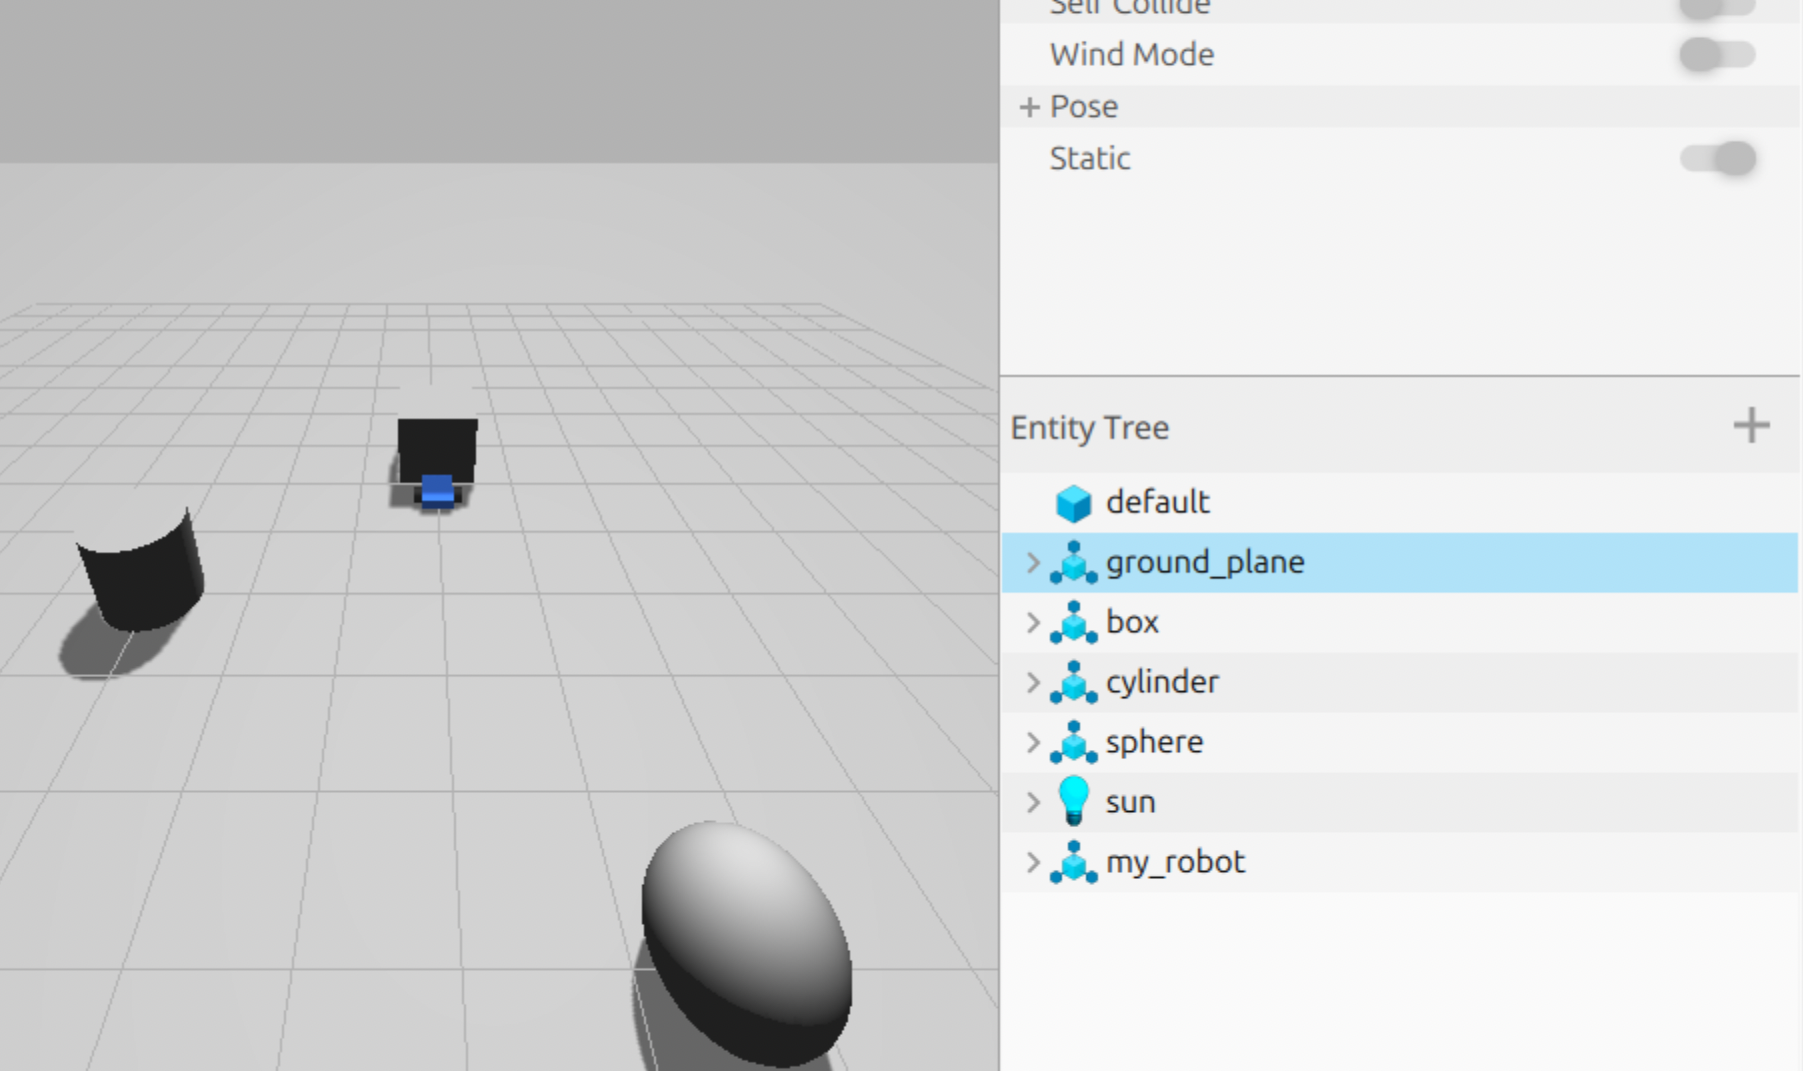
\includegraphics[width=\columnwidth]{fig/Task2/04_GzSimKeyboard.png}
    \caption{The robot driving in the custom world under keyboard control.}
    \label{fig:t2_driving}
\end{figure}

\begin{figure}[H]
    \centering
    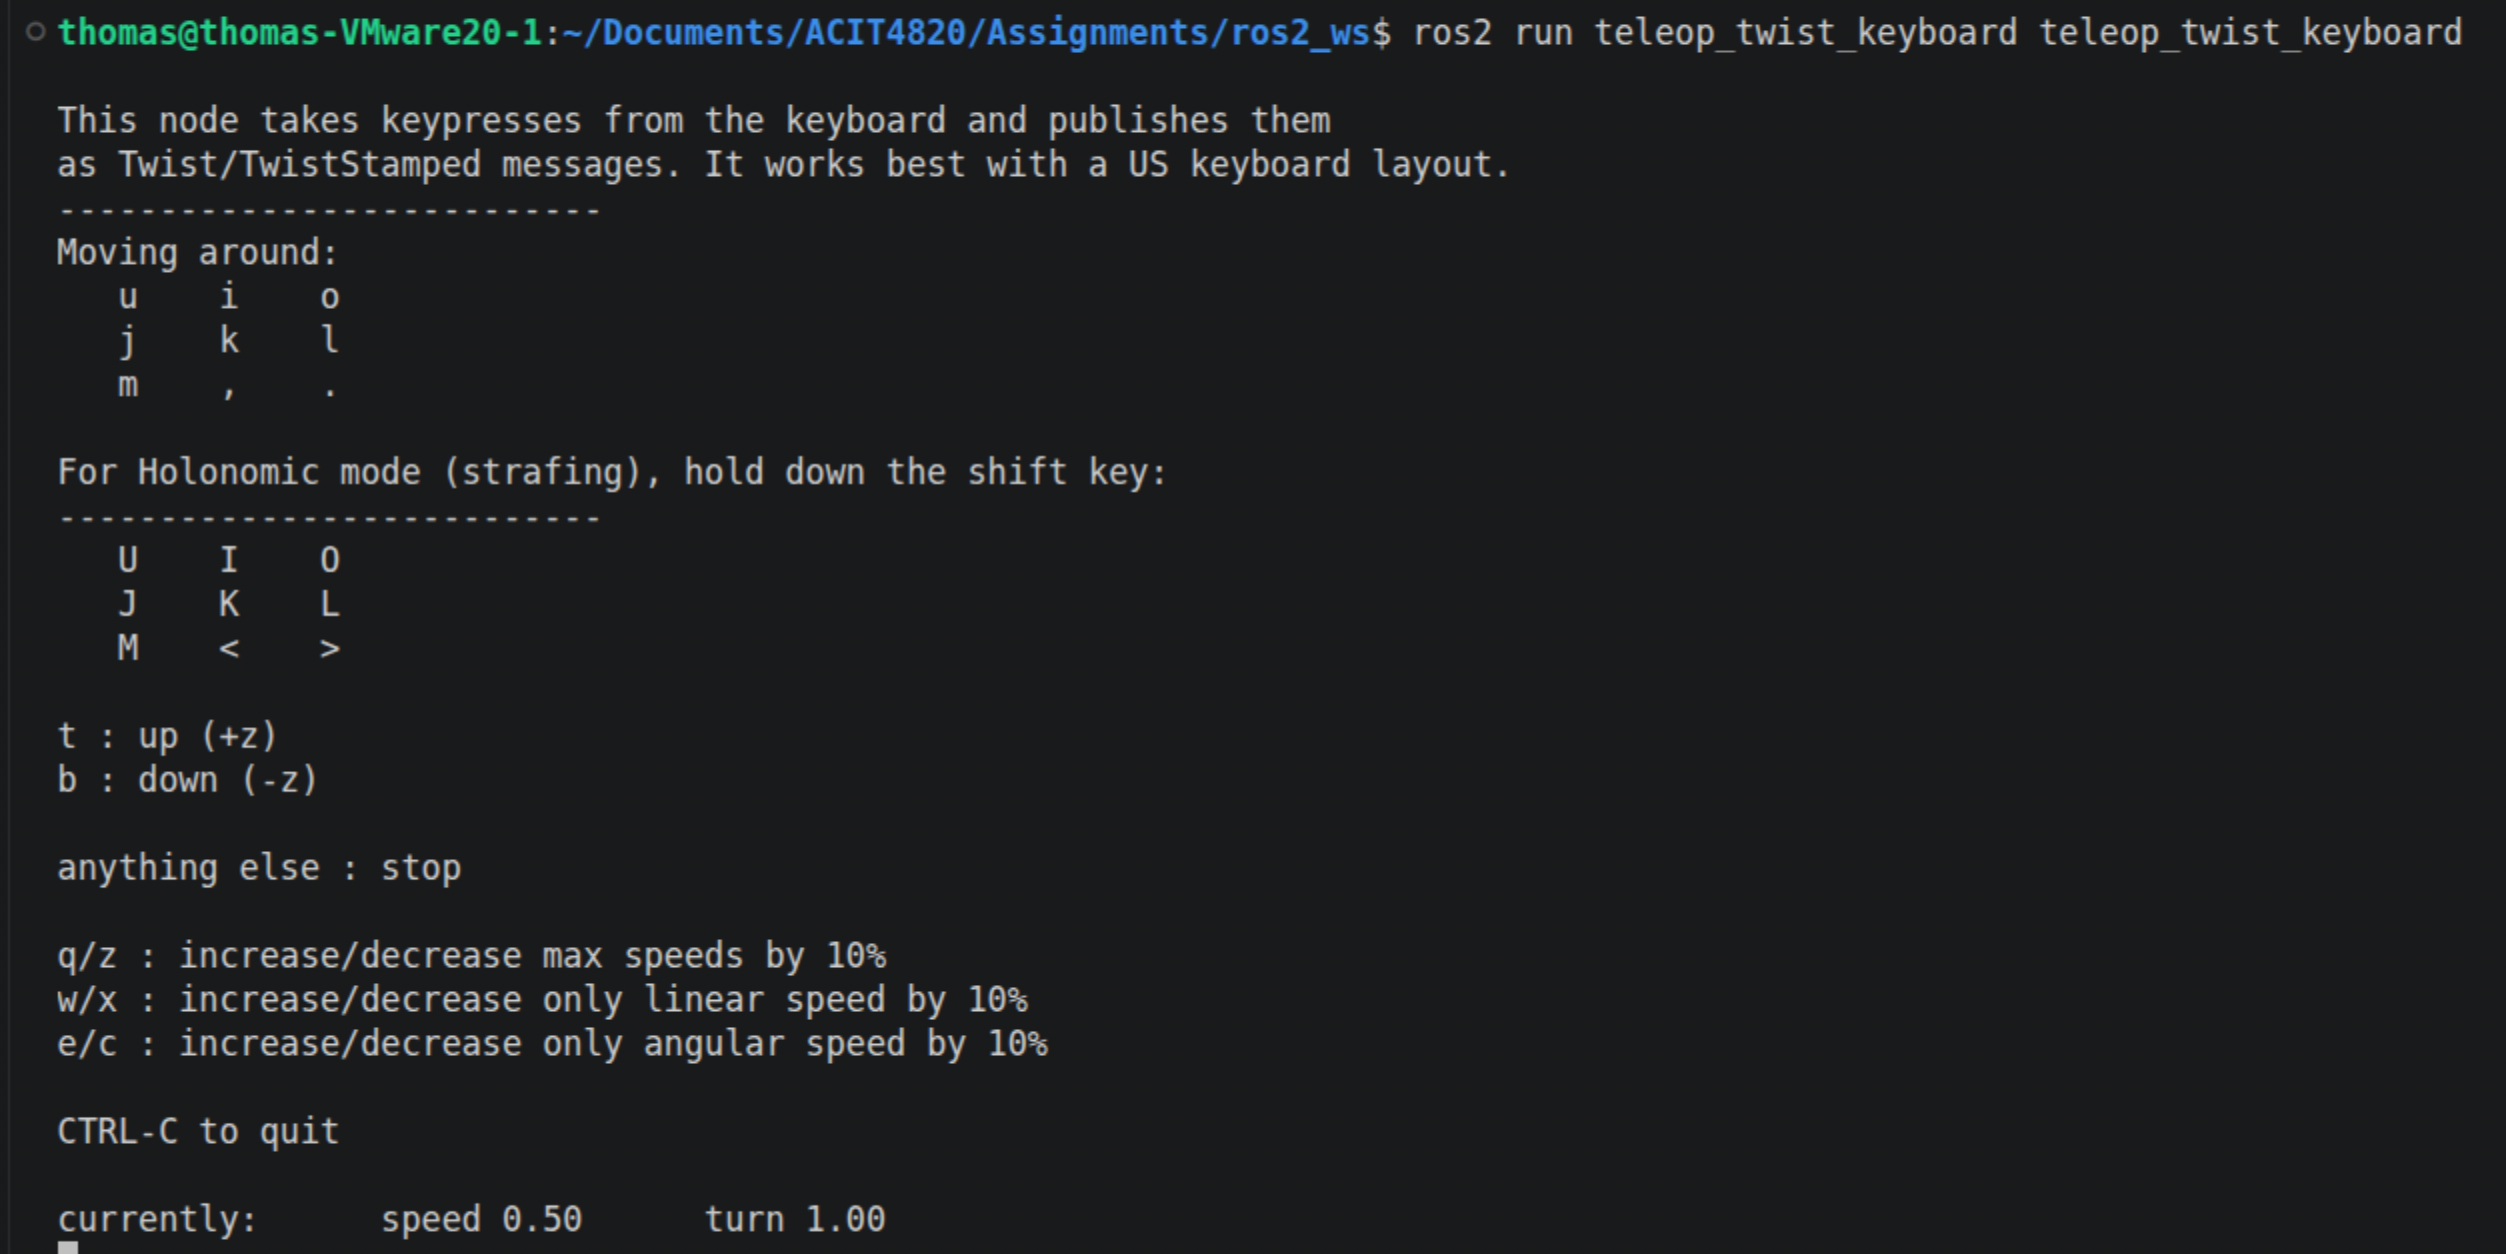
\includegraphics[width=\columnwidth]{fig/Task2/02_KeyboardThernimal.png}
    \caption{The teleop\_twist\_keyboard node running.}
    \label{fig:t2_teleop}
\end{figure}

\begin{figure}[H]
    \centering
    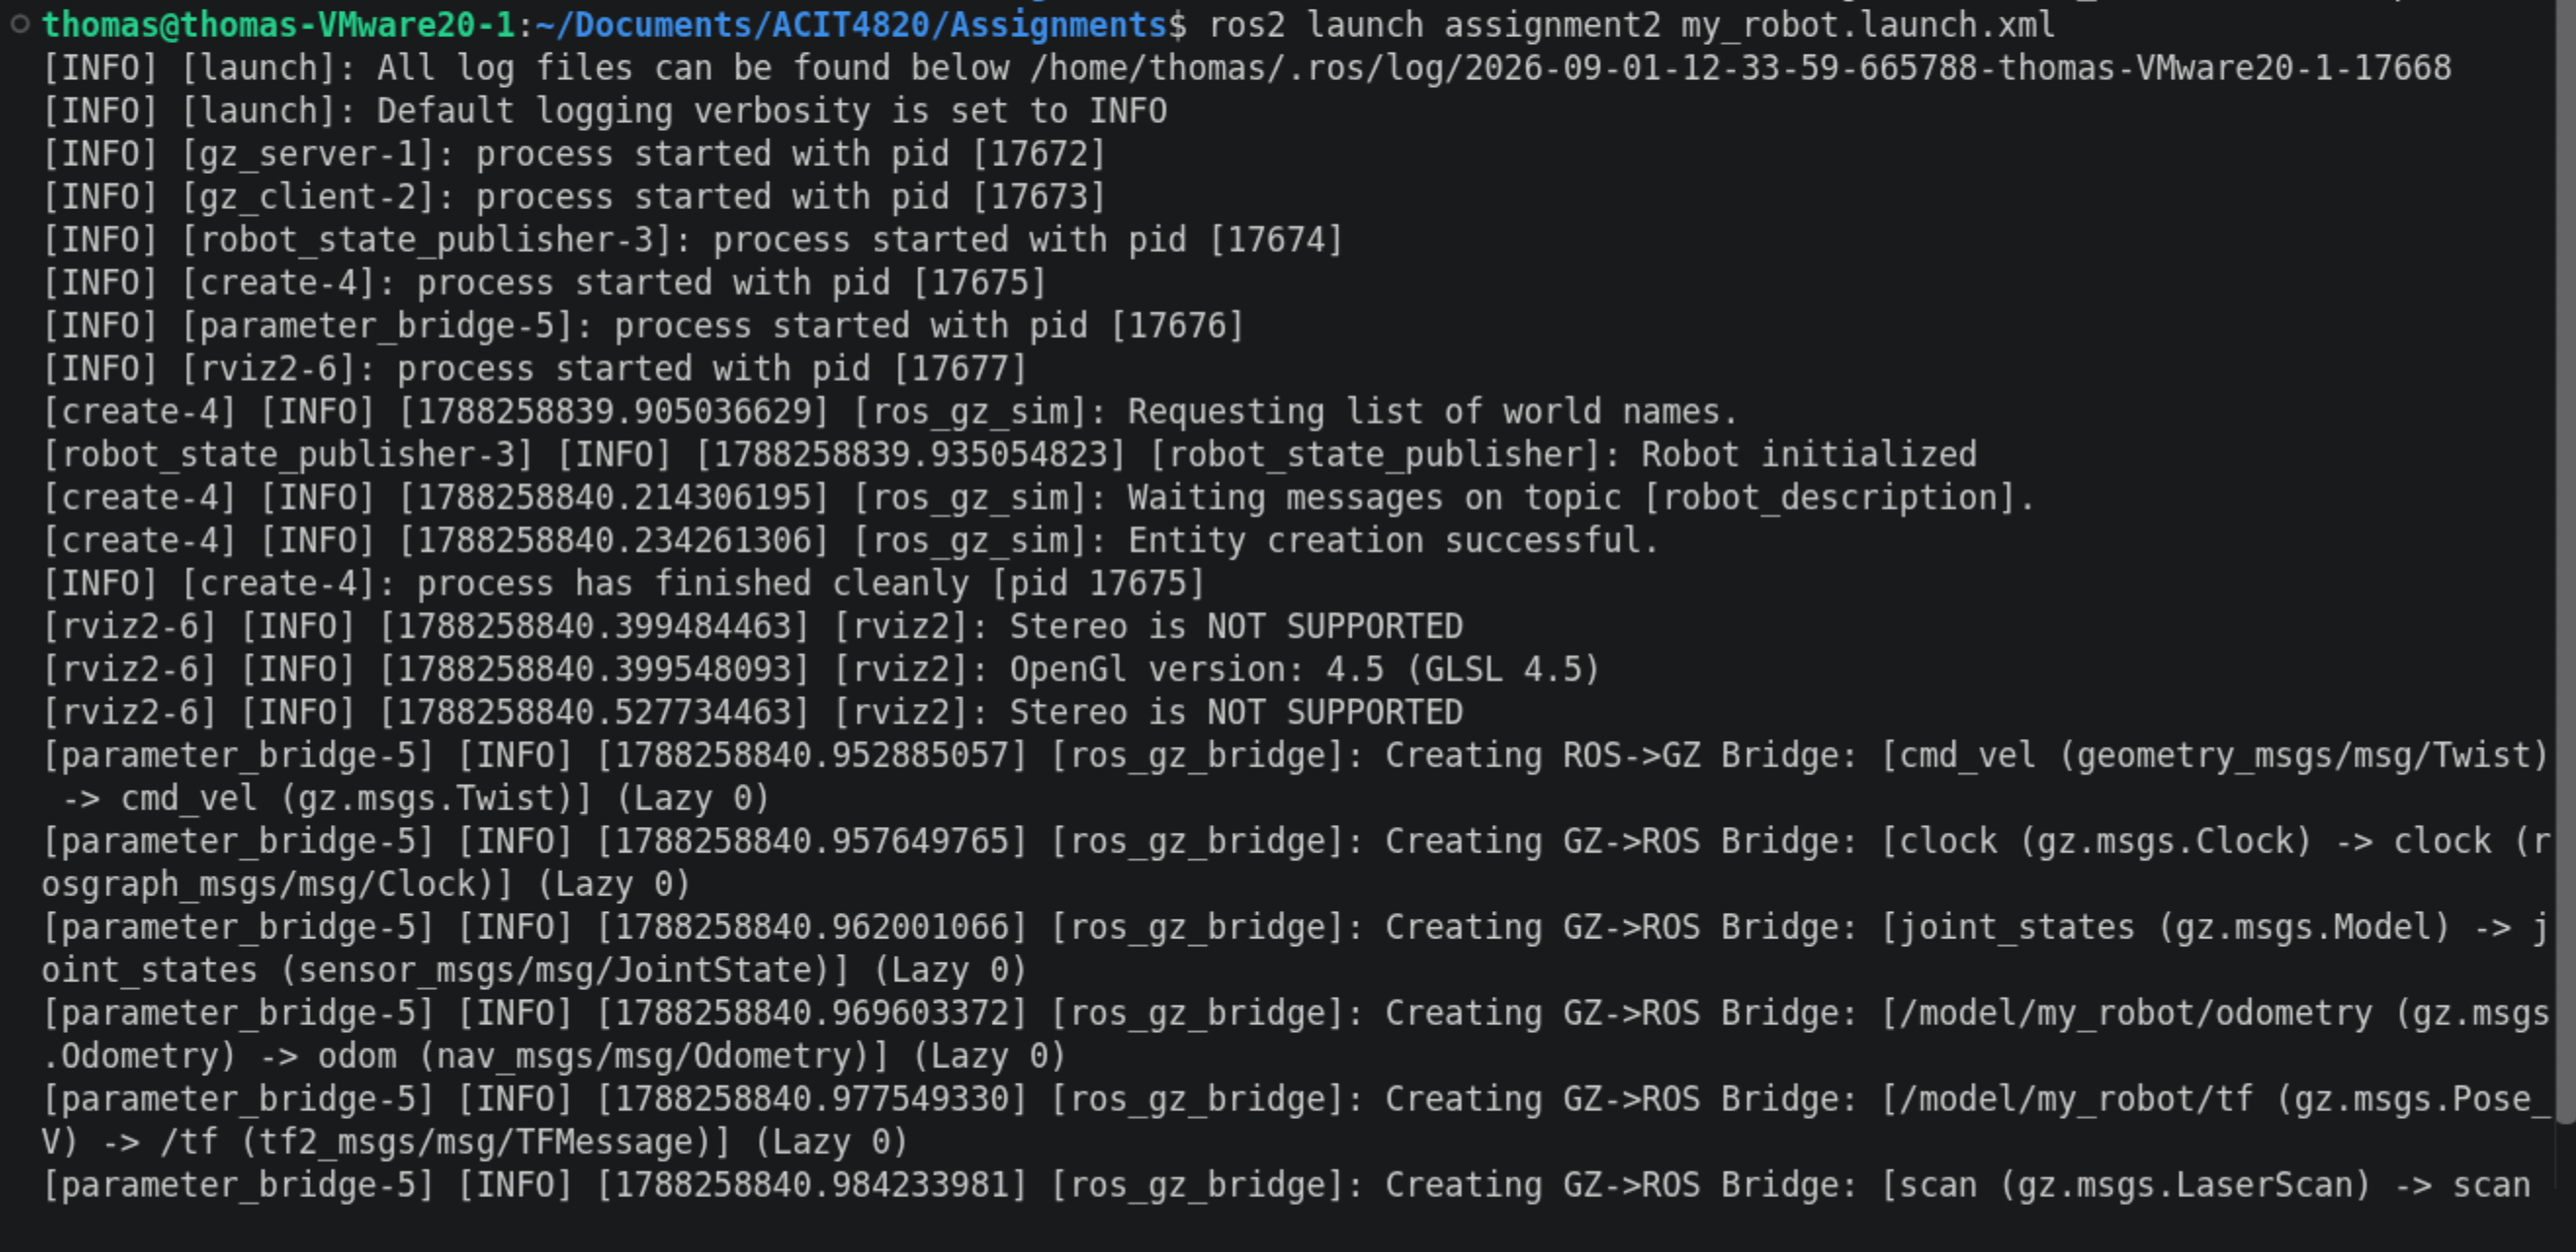
\includegraphics[width=\columnwidth]{fig/Task2/03_KeyboardLaunch.png}
    \caption{The launch file bringing up Gazebo, the robot, the bridge and
             RViz together.}
    \label{fig:t2_launch}
\end{figure}

\begin{figure}[H]
    \centering
    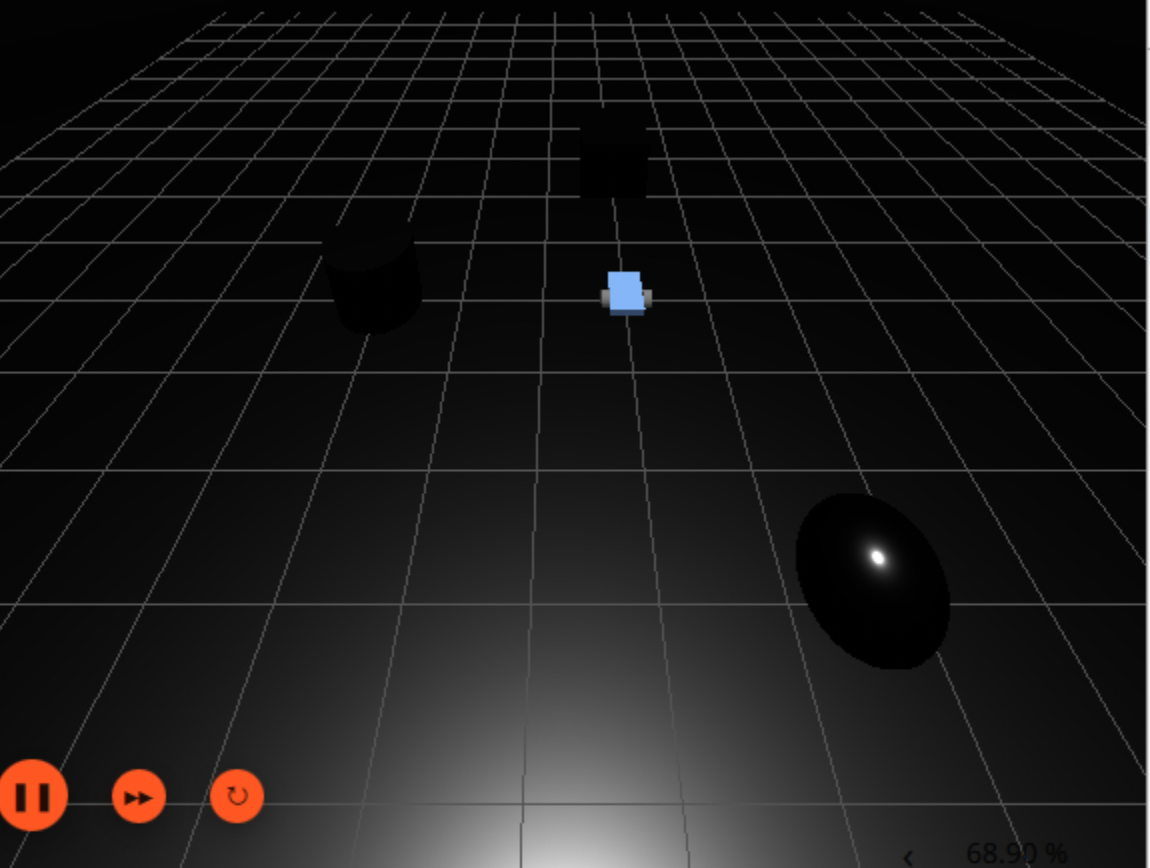
\includegraphics[width=\columnwidth]{fig/Task2/00_task2darkworld.png}
    \caption{The world before the lighting and render engine were fixed. The
             file validated and every plugin loaded, but the obstacles
             rendered as black silhouettes.}
    \label{fig:t2_dark}
\end{figure}

\begin{figure}[H]
    \centering
    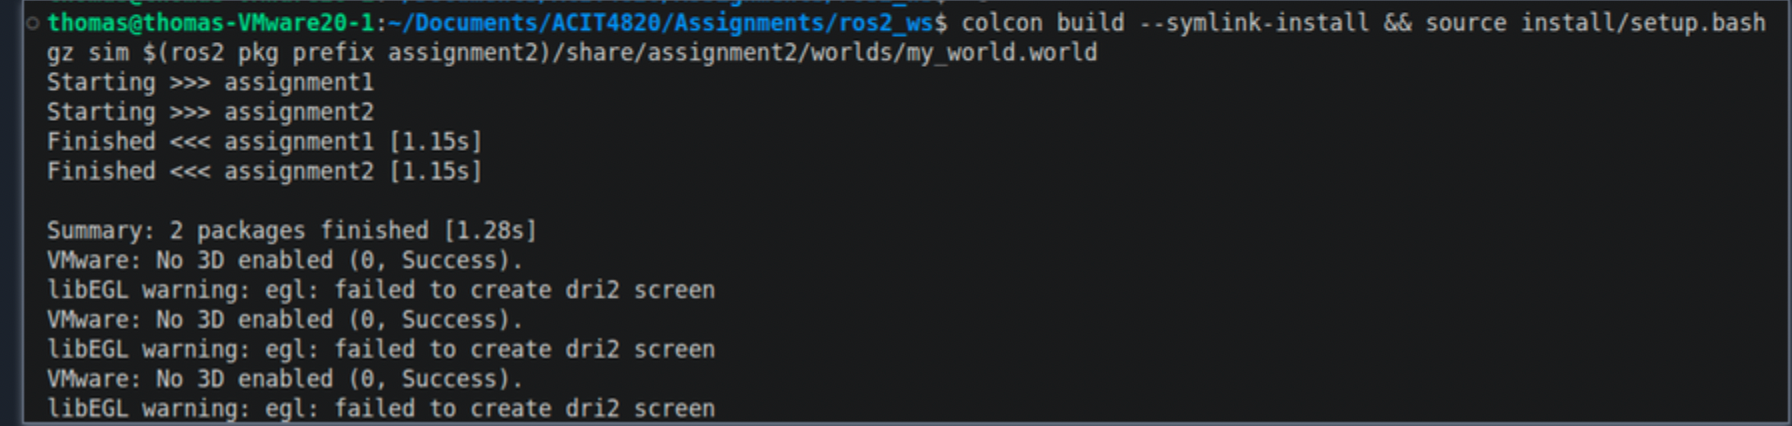
\includegraphics[width=\columnwidth]{fig/Task2/01_taskWordlDarkTerminal.png}
    \caption{Terminal output while the world rendered black. The build
             succeeds, but Gazebo reports that 3D is not enabled and that EGL
             failed to create a screen.}
    \label{fig:t2_darkterm}
\end{figure}

\subsection*{Task 3: LiDAR sensor}

The sensor sits inside a gazebo tag on lidar\_link, which URDF ignores and
Gazebo reads. The gz\_frame\_id line is what stamps the scan with lidar\_link
so RViz can place the points, and the scan angles are the values used in the
Gazebo documentation.

\begin{listing}[H]
\begin{minted}{xml}
<sensor name="lidar" type="gpu_lidar">
  <topic>scan</topic>
  <gz_frame_id>lidar_link</gz_frame_id>
  <update_rate>10</update_rate>
  <always_on>1</always_on>
  <visualize>true</visualize>
  <ray>
    <scan>
      <horizontal>
        <samples>640</samples>
        <min_angle>-1.396263</min_angle>
        <max_angle>1.396263</max_angle>
      </horizontal>
    </scan>
    <range>
      <min>0.08</min>
      <max>10.0</max>
    </range>
  </ray>
</sensor>
\end{minted}
\caption{The LiDAR sensor block, from lidar.xacro. The single row vertical
         scan and the resolution fields are left out for brevity.}
\label{lst:lidar}
\end{listing}

\begin{figure}[H]
    \centering
    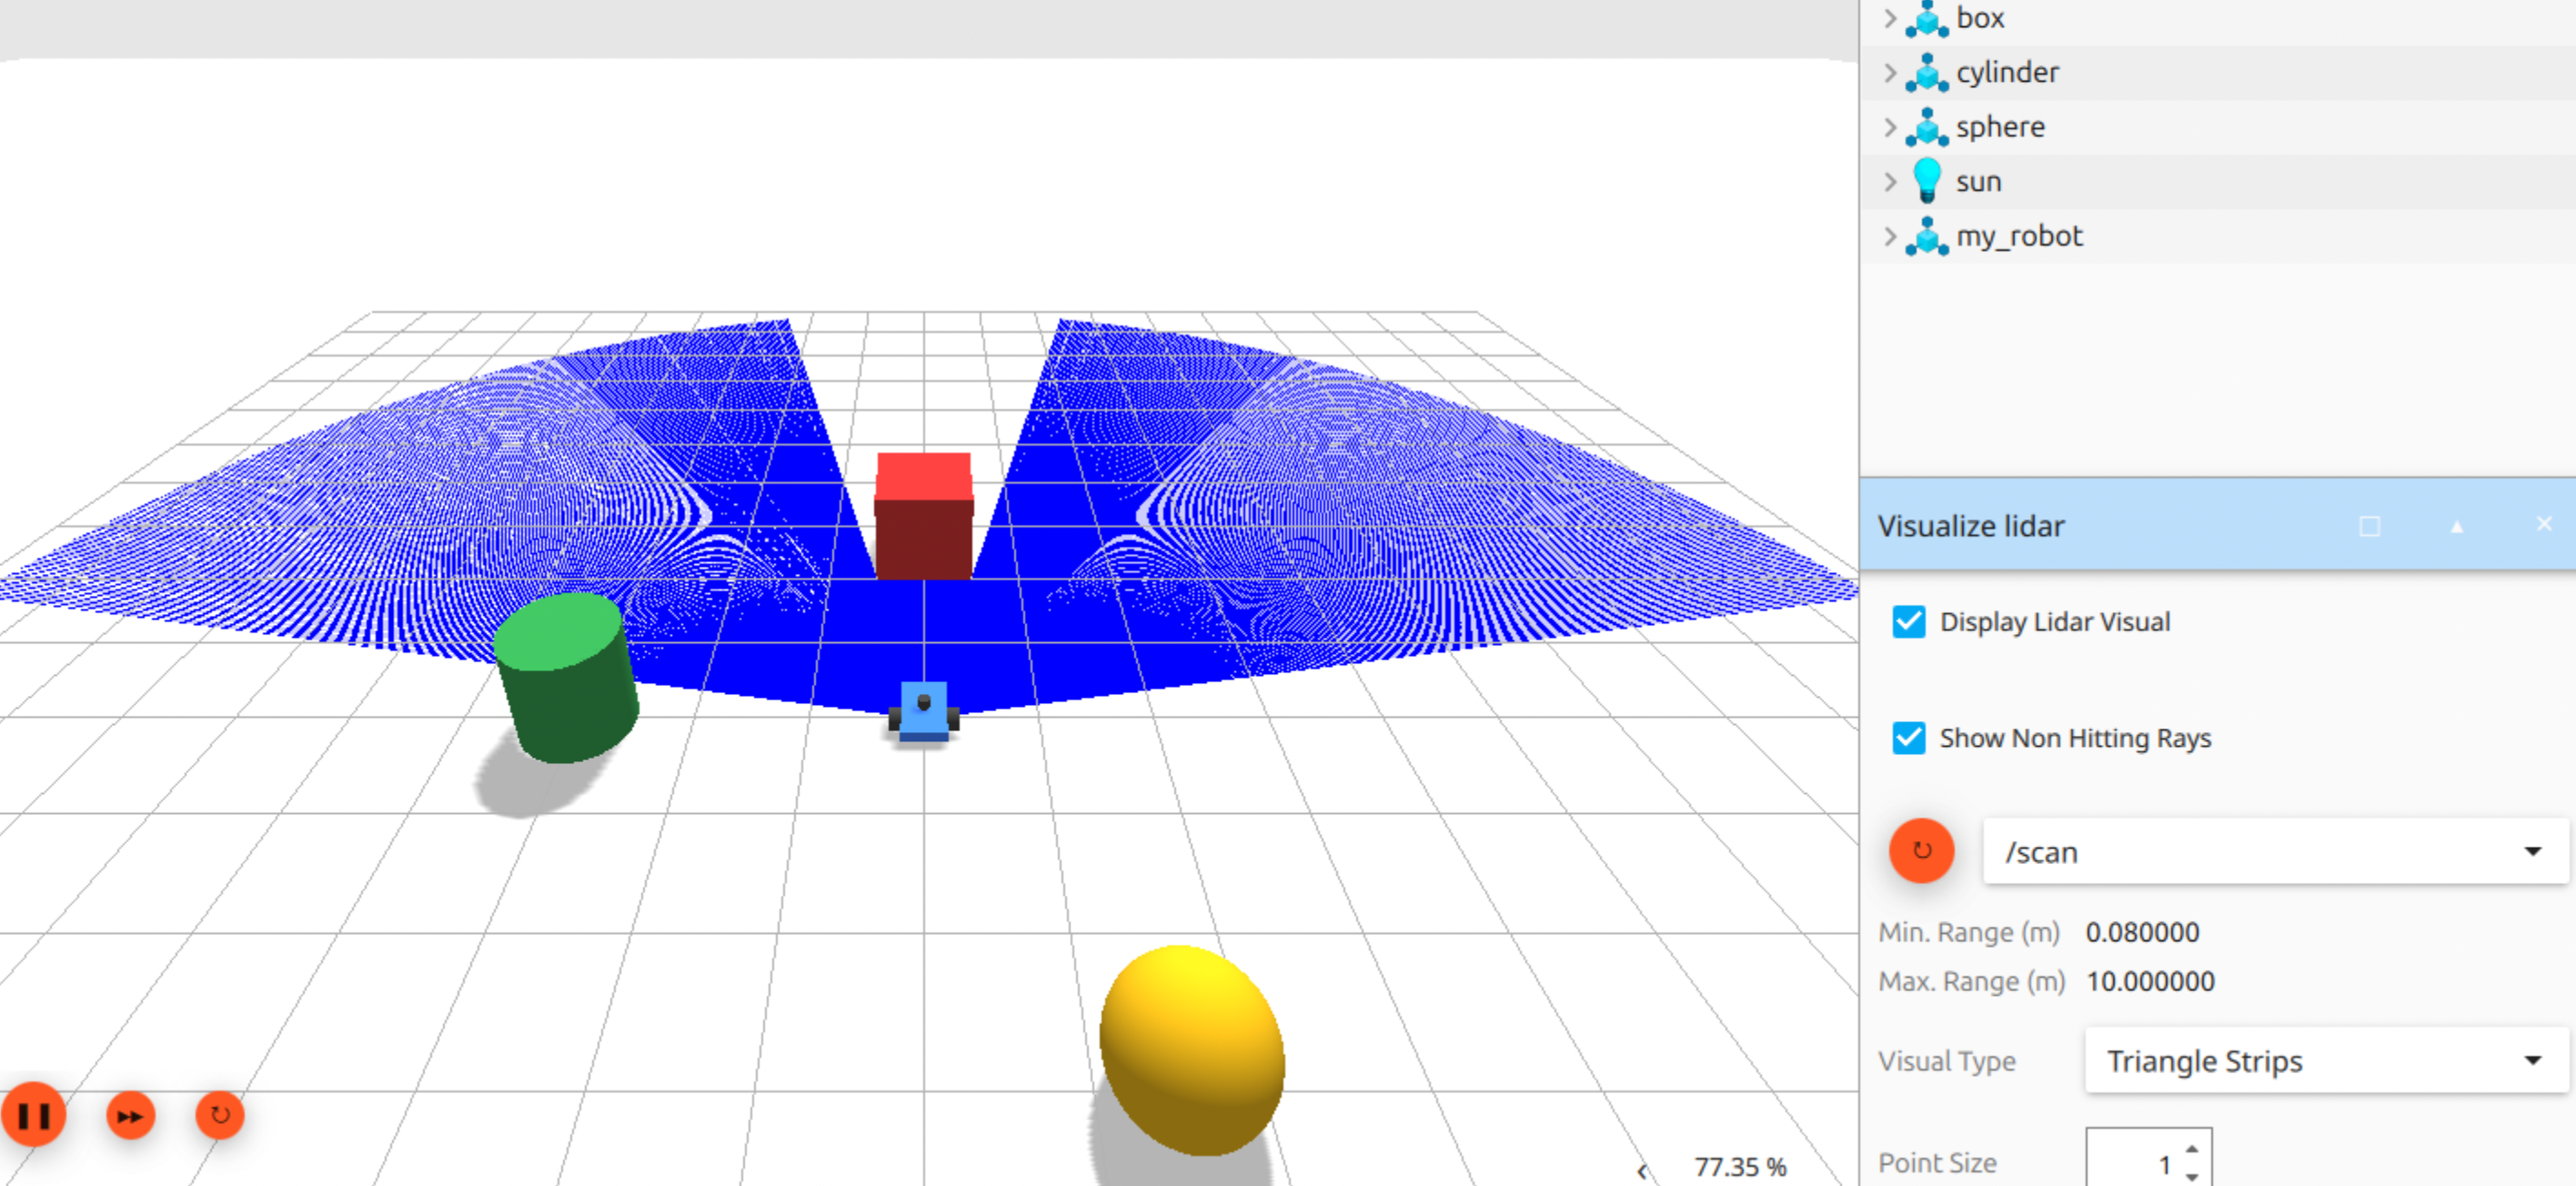
\includegraphics[width=\columnwidth]{fig/Task3/01_GzRadar.png}
    \caption{The LiDAR visualised in Gazebo. The rays stop at the box and leave
             a shadow behind it, showing genuine line of sight occlusion.}
    \label{fig:t3_gazebo}
\end{figure}

\begin{figure}[H]
    \centering
    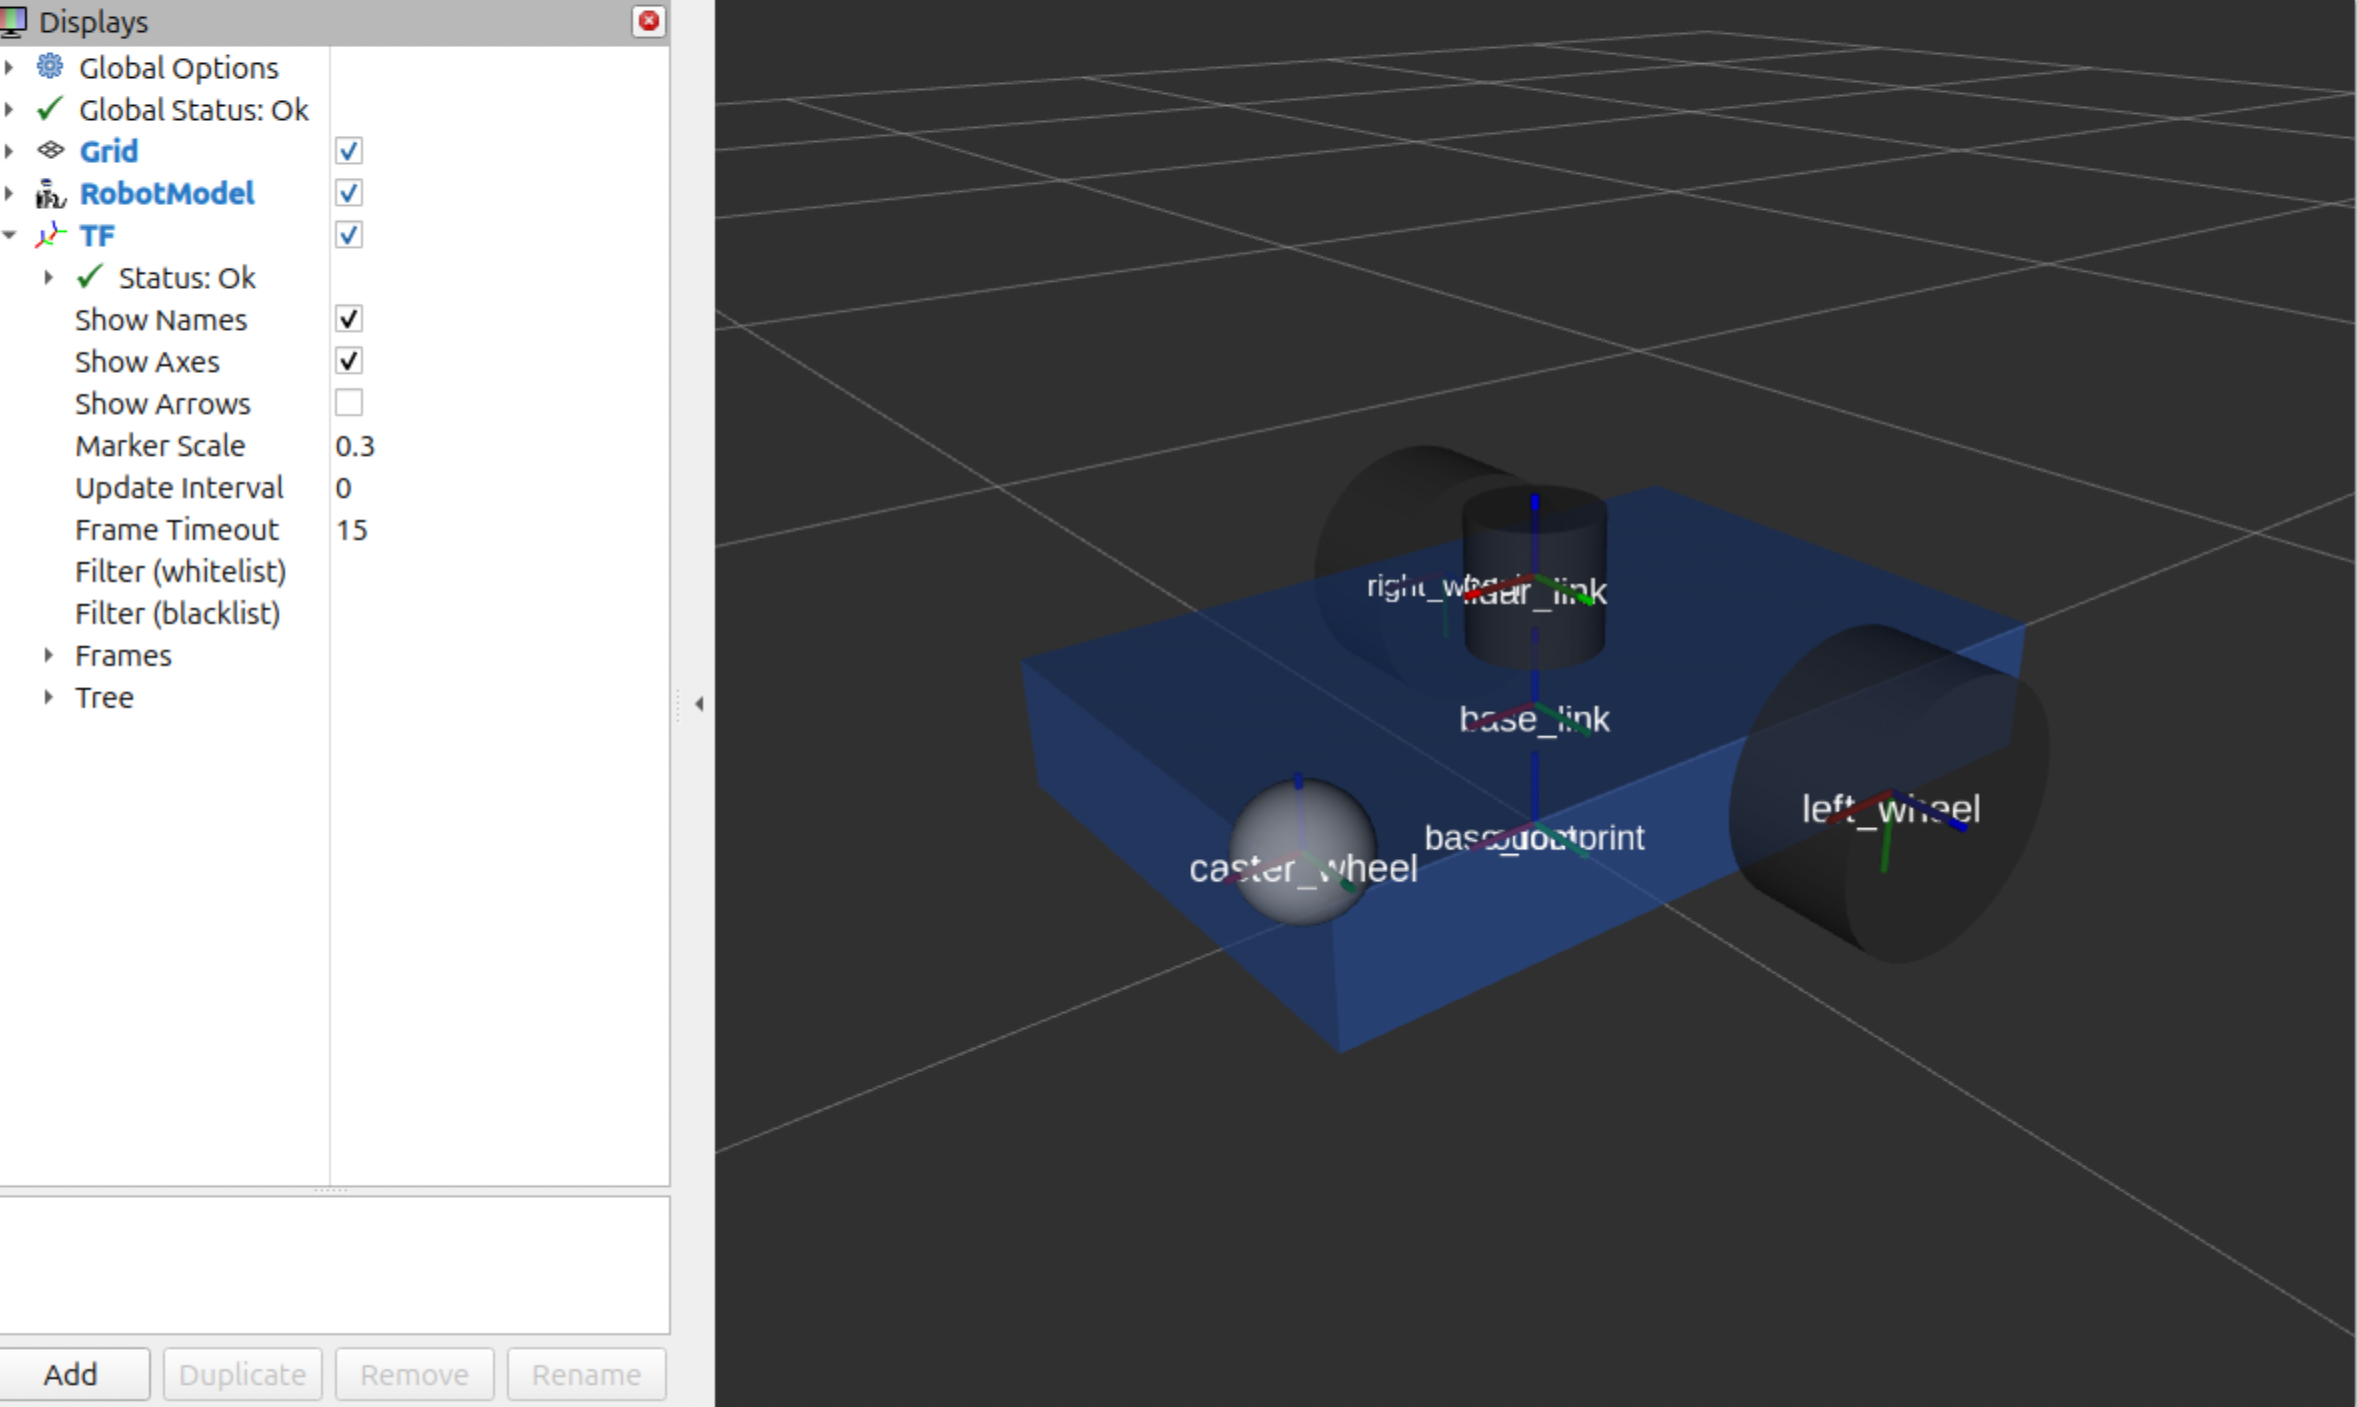
\includegraphics[width=\columnwidth]{fig/Task3/00_RadarVisual.png}
    \caption{Our first configuration, a full 360 degree scan. We later changed
             this to the 640 samples over plus minus 80 degrees used in the
             Gazebo documentation.}
    \label{fig:t3_360}
\end{figure}

\begin{figure}[H]
    \centering
    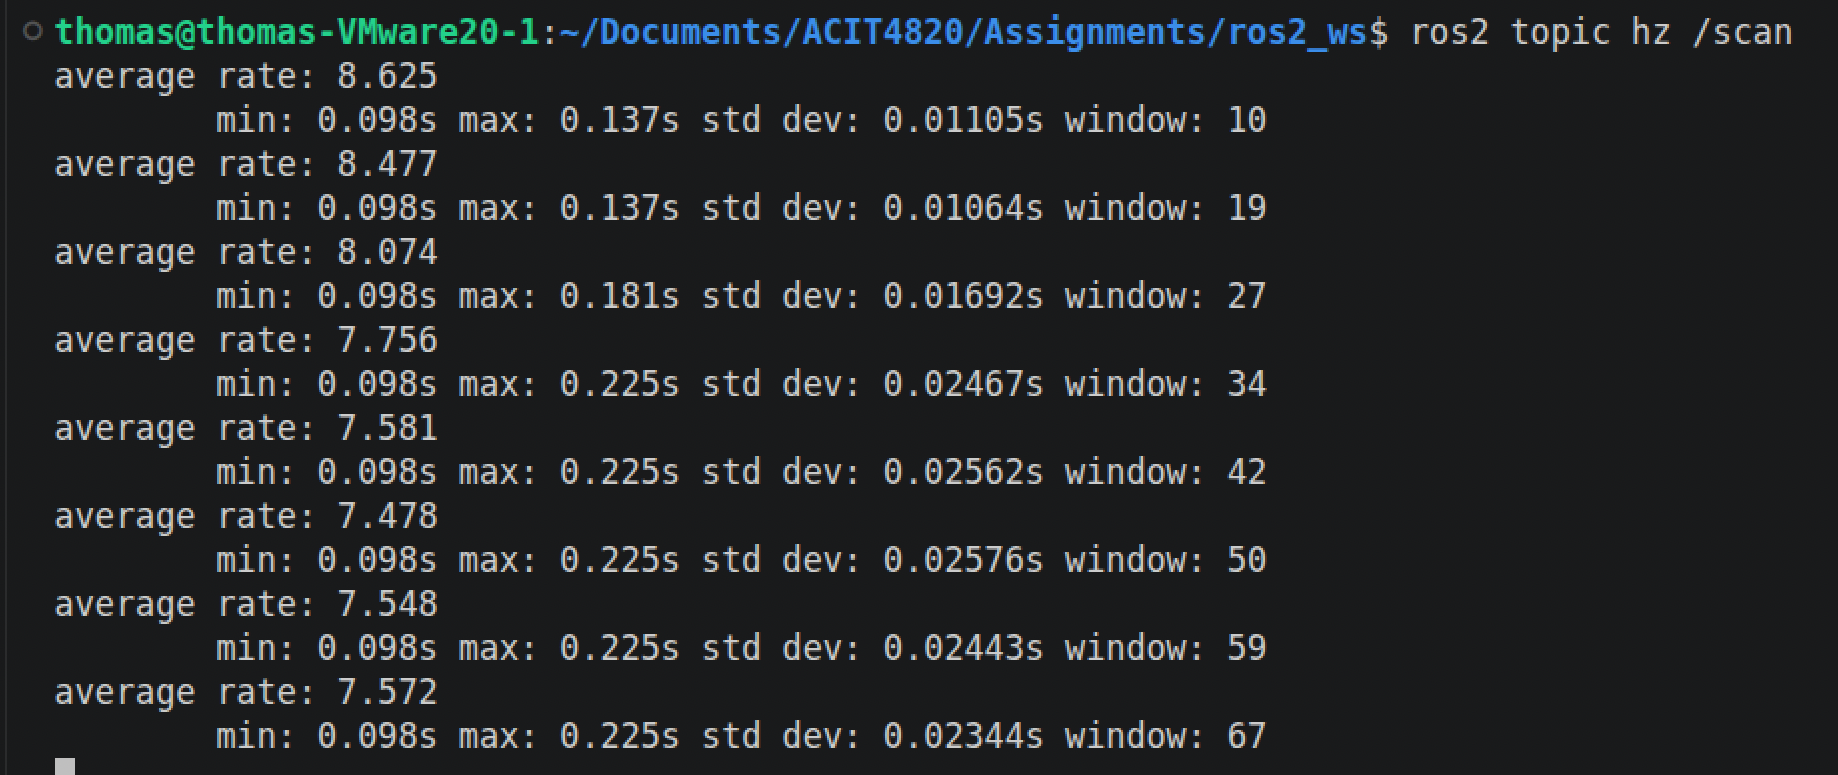
\includegraphics[width=\columnwidth]{fig/Task3/02_GzRadarTerminal.png}
    \caption{The scan publishing to ROS at around 8 Hz, which is the 10 Hz
             sensor rate scaled by the simulation's real time factor.}
    \label{fig:t3_hz}
\end{figure}

\begin{figure}[H]
    \centering
    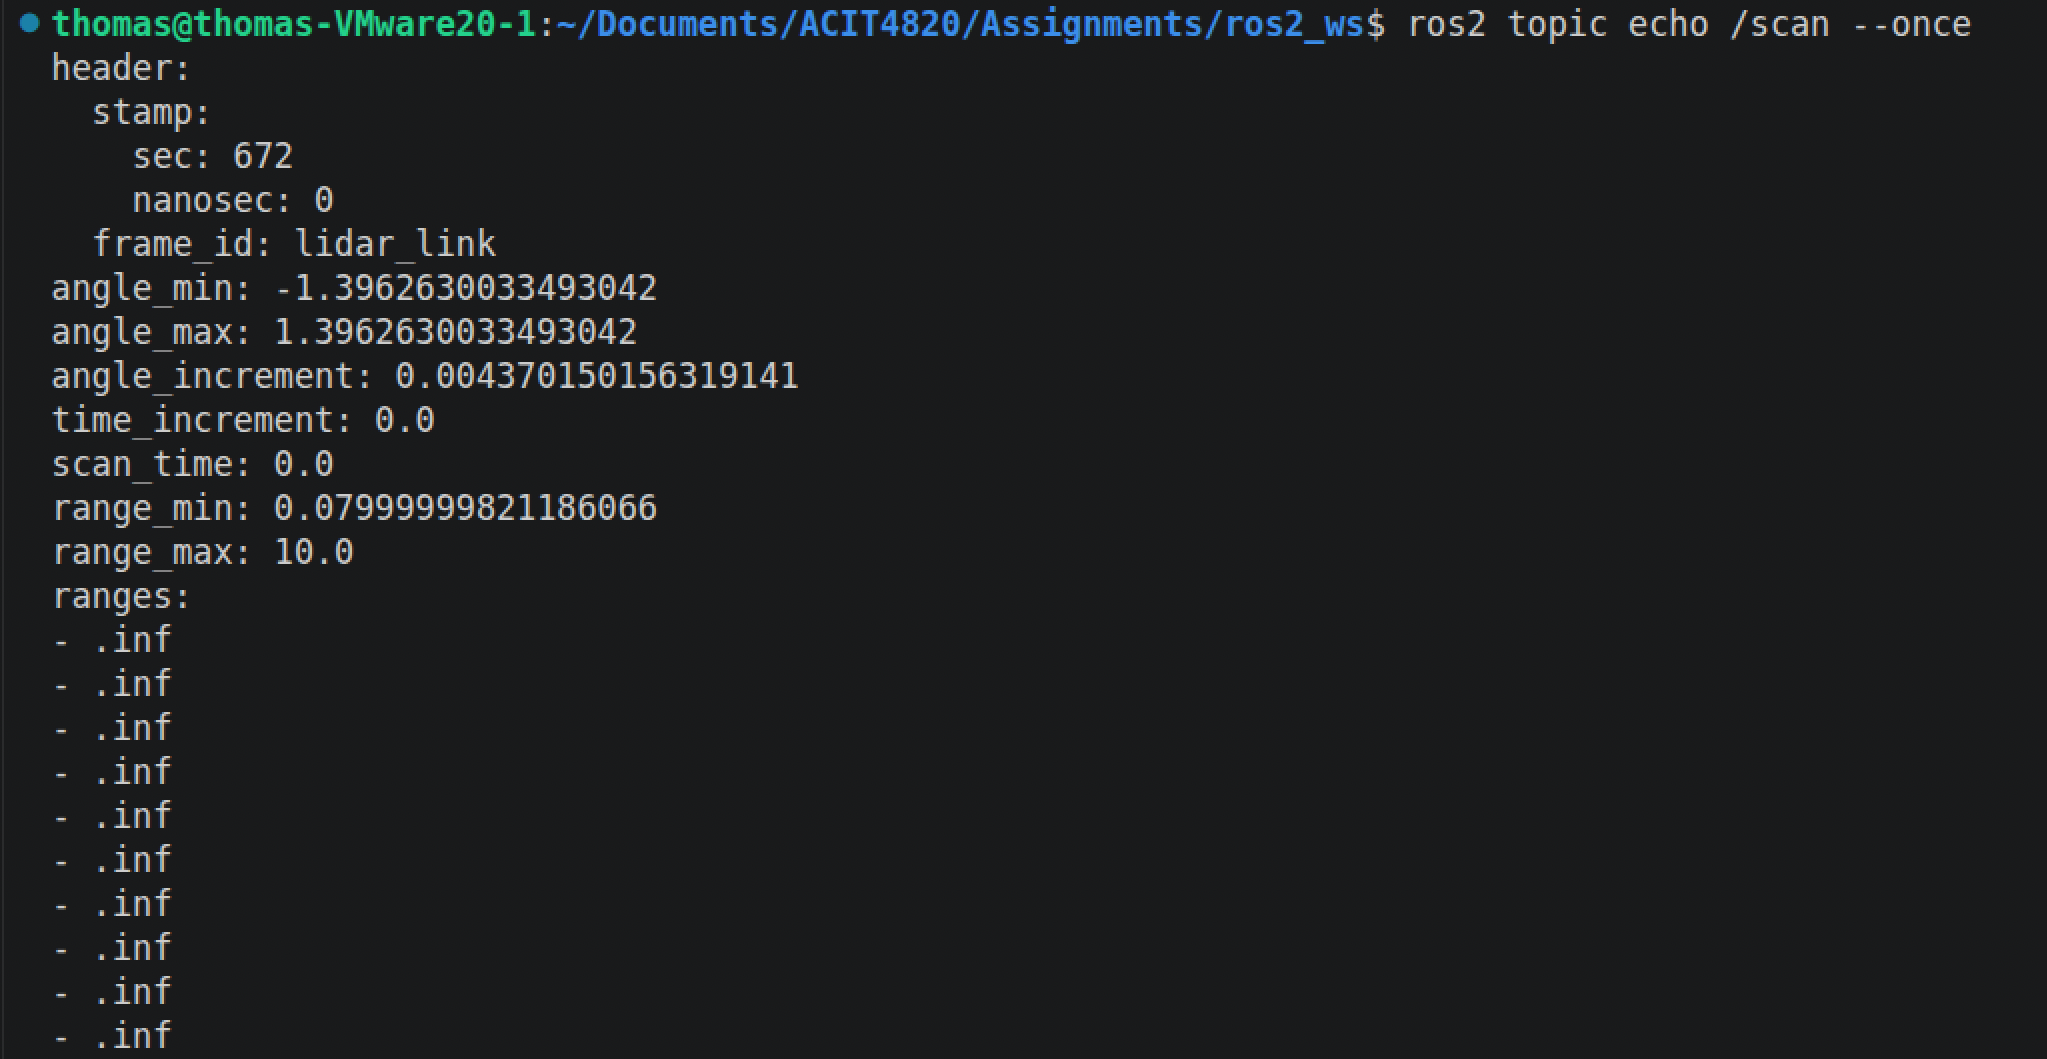
\includegraphics[width=\columnwidth]{fig/Task3/03_GzRadarTerminal2.png}
    \caption{One scan message on the ROS side, confirming the frame is
             lidar\_link and the angles match the configuration.}
    \label{fig:t3_echo}
\end{figure}

\subsection*{Task 4: Visualising the scan in RViz}

\begin{figure}[H]
    \centering
    \begin{subfigure}{\columnwidth}
        \centering
        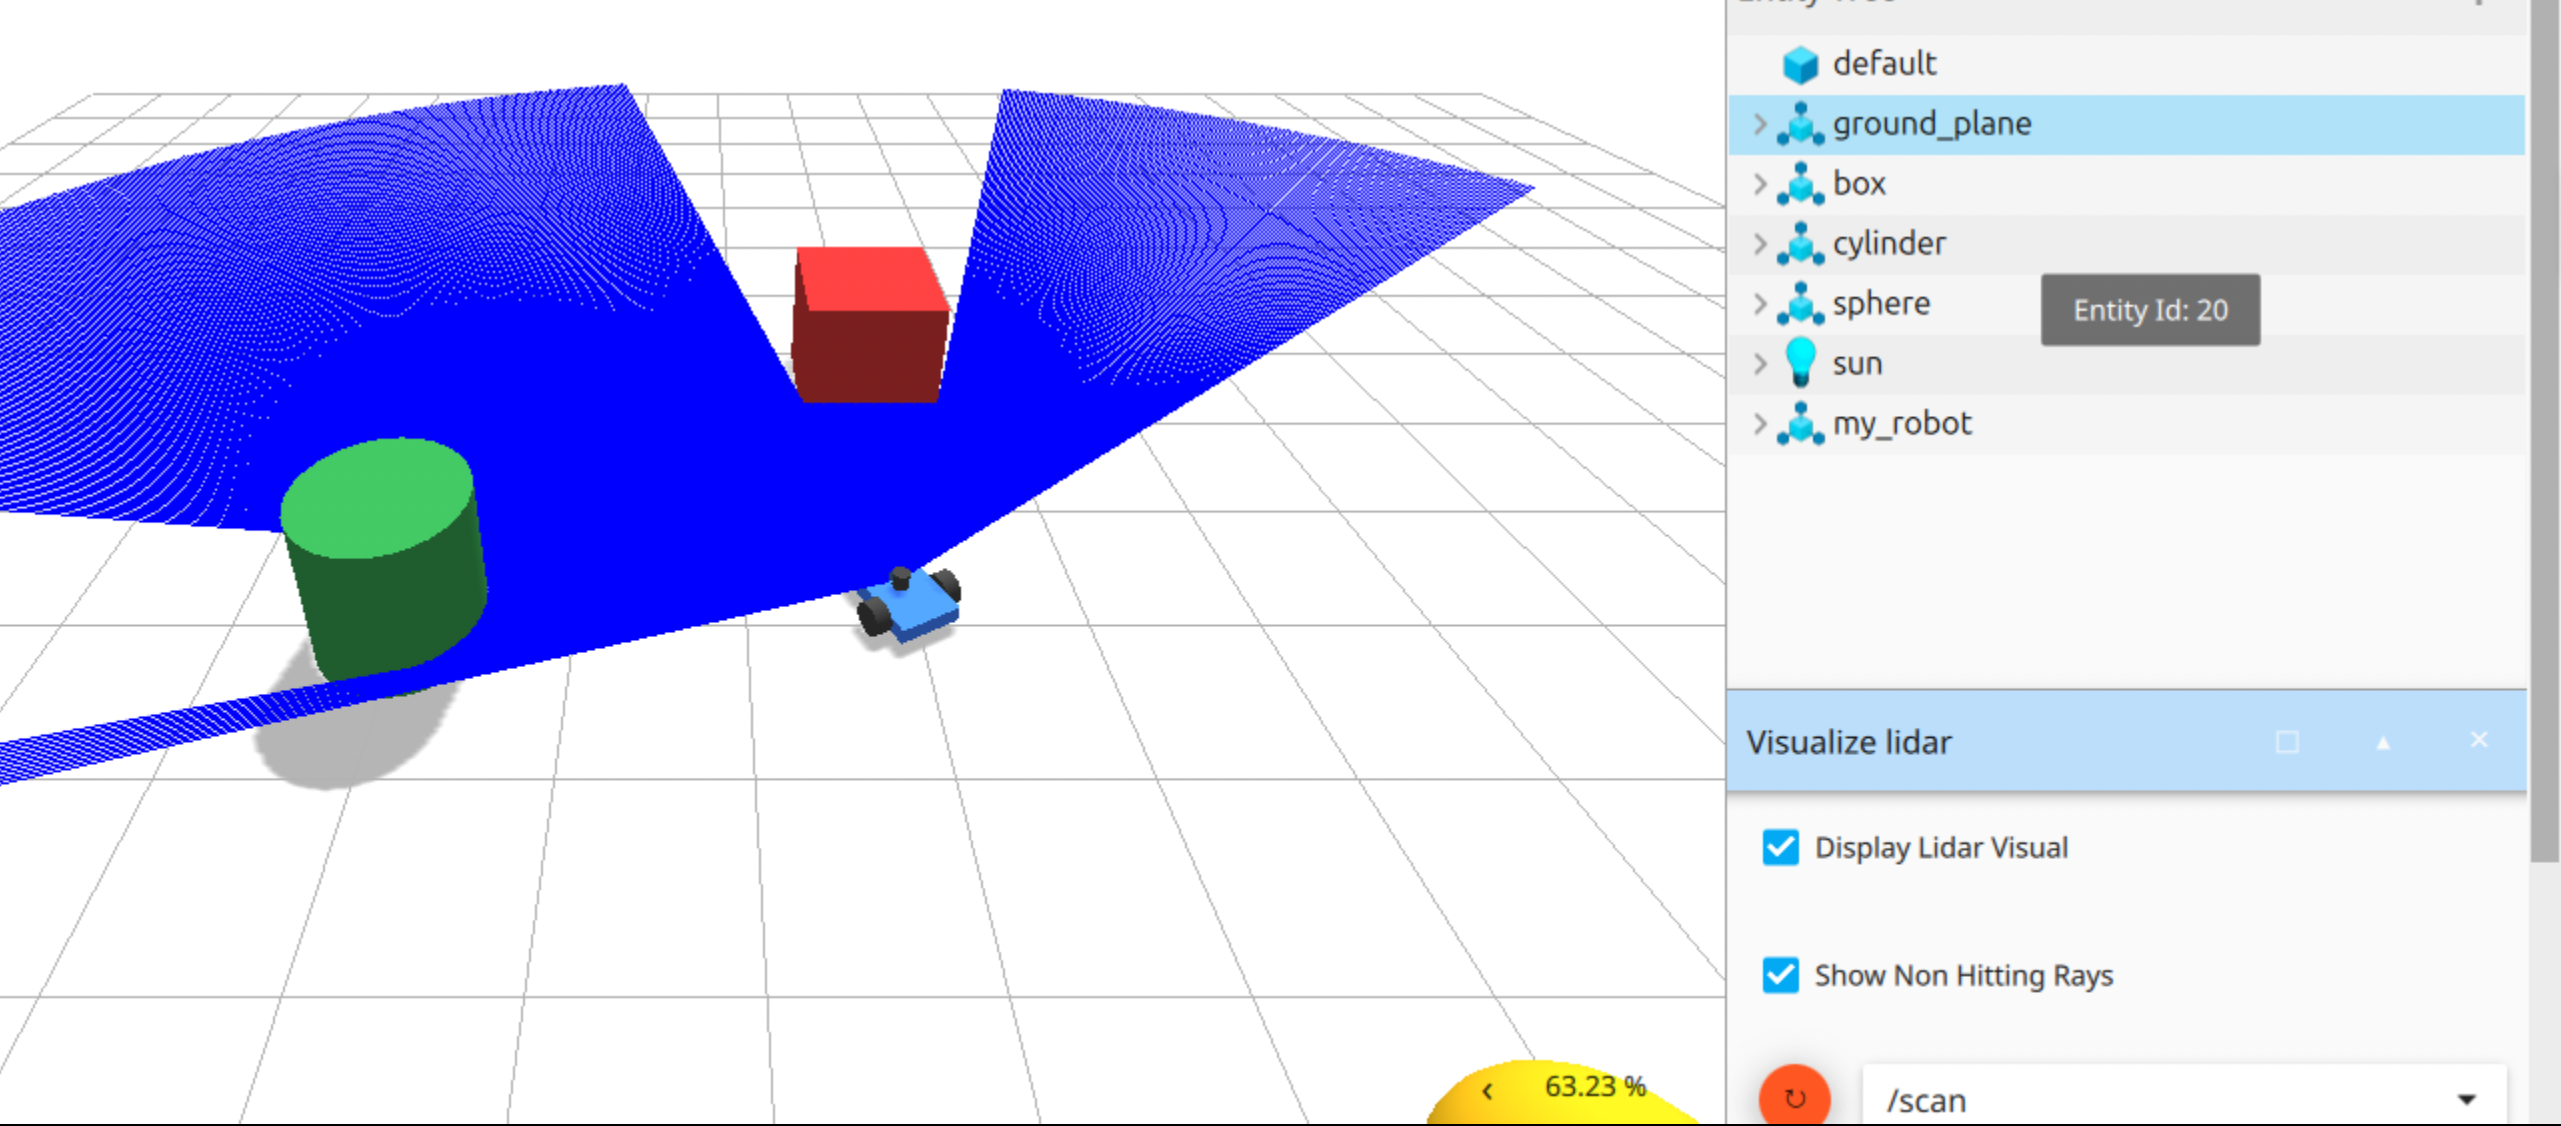
\includegraphics[width=\linewidth]{fig/Task4/00_scanGz.png}
        \caption{Gazebo}
    \end{subfigure}
    \\[6pt]
    \begin{subfigure}{\columnwidth}
        \centering
        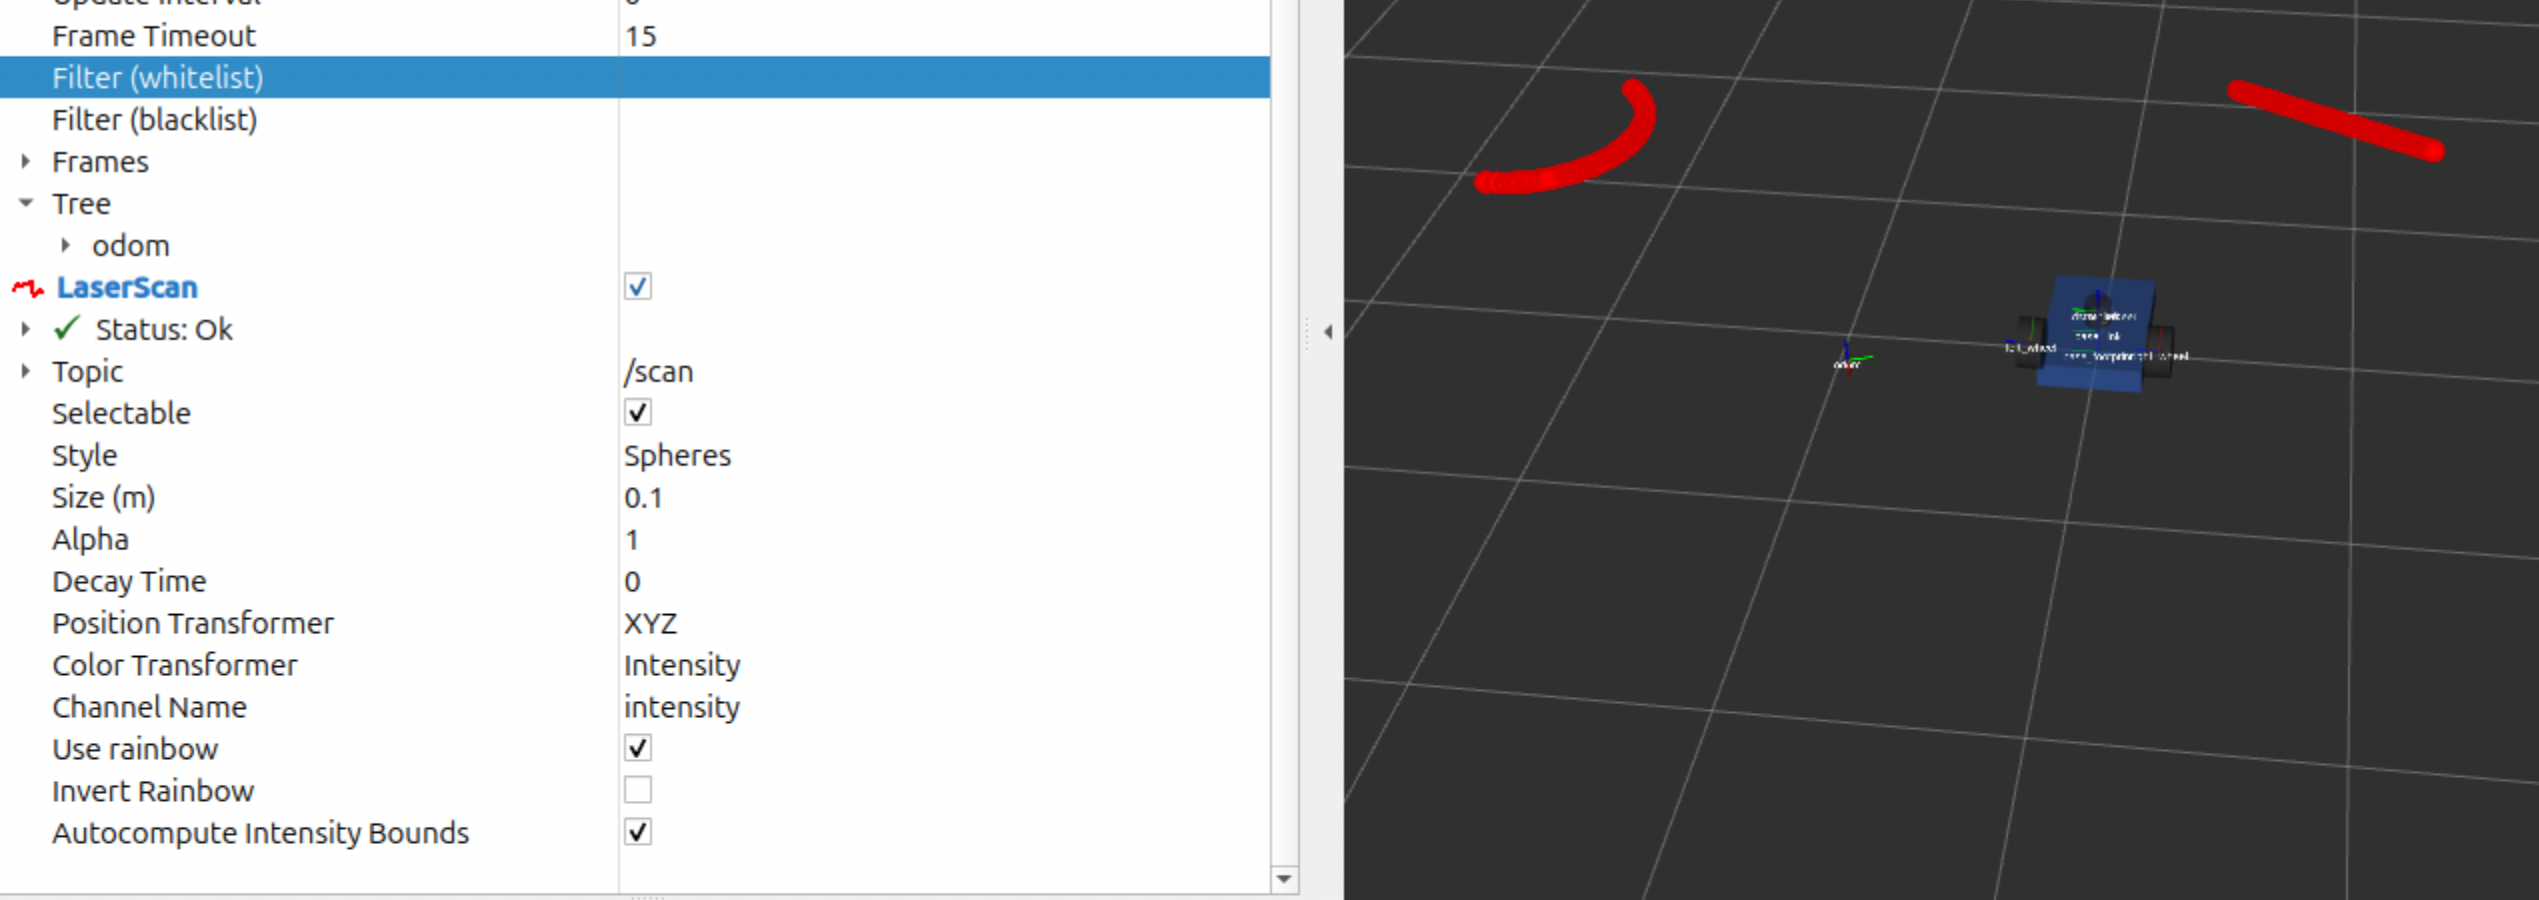
\includegraphics[width=\linewidth]{fig/Task4/01_scanRivz.png}
        \caption{RViz}
    \end{subfigure}
    \caption{The robot at a distance from the box, with the corresponding laser
             scan in RViz.}
    \label{fig:t4_far}
\end{figure}

\begin{figure}[H]
    \centering
    \begin{subfigure}{\columnwidth}
        \centering
        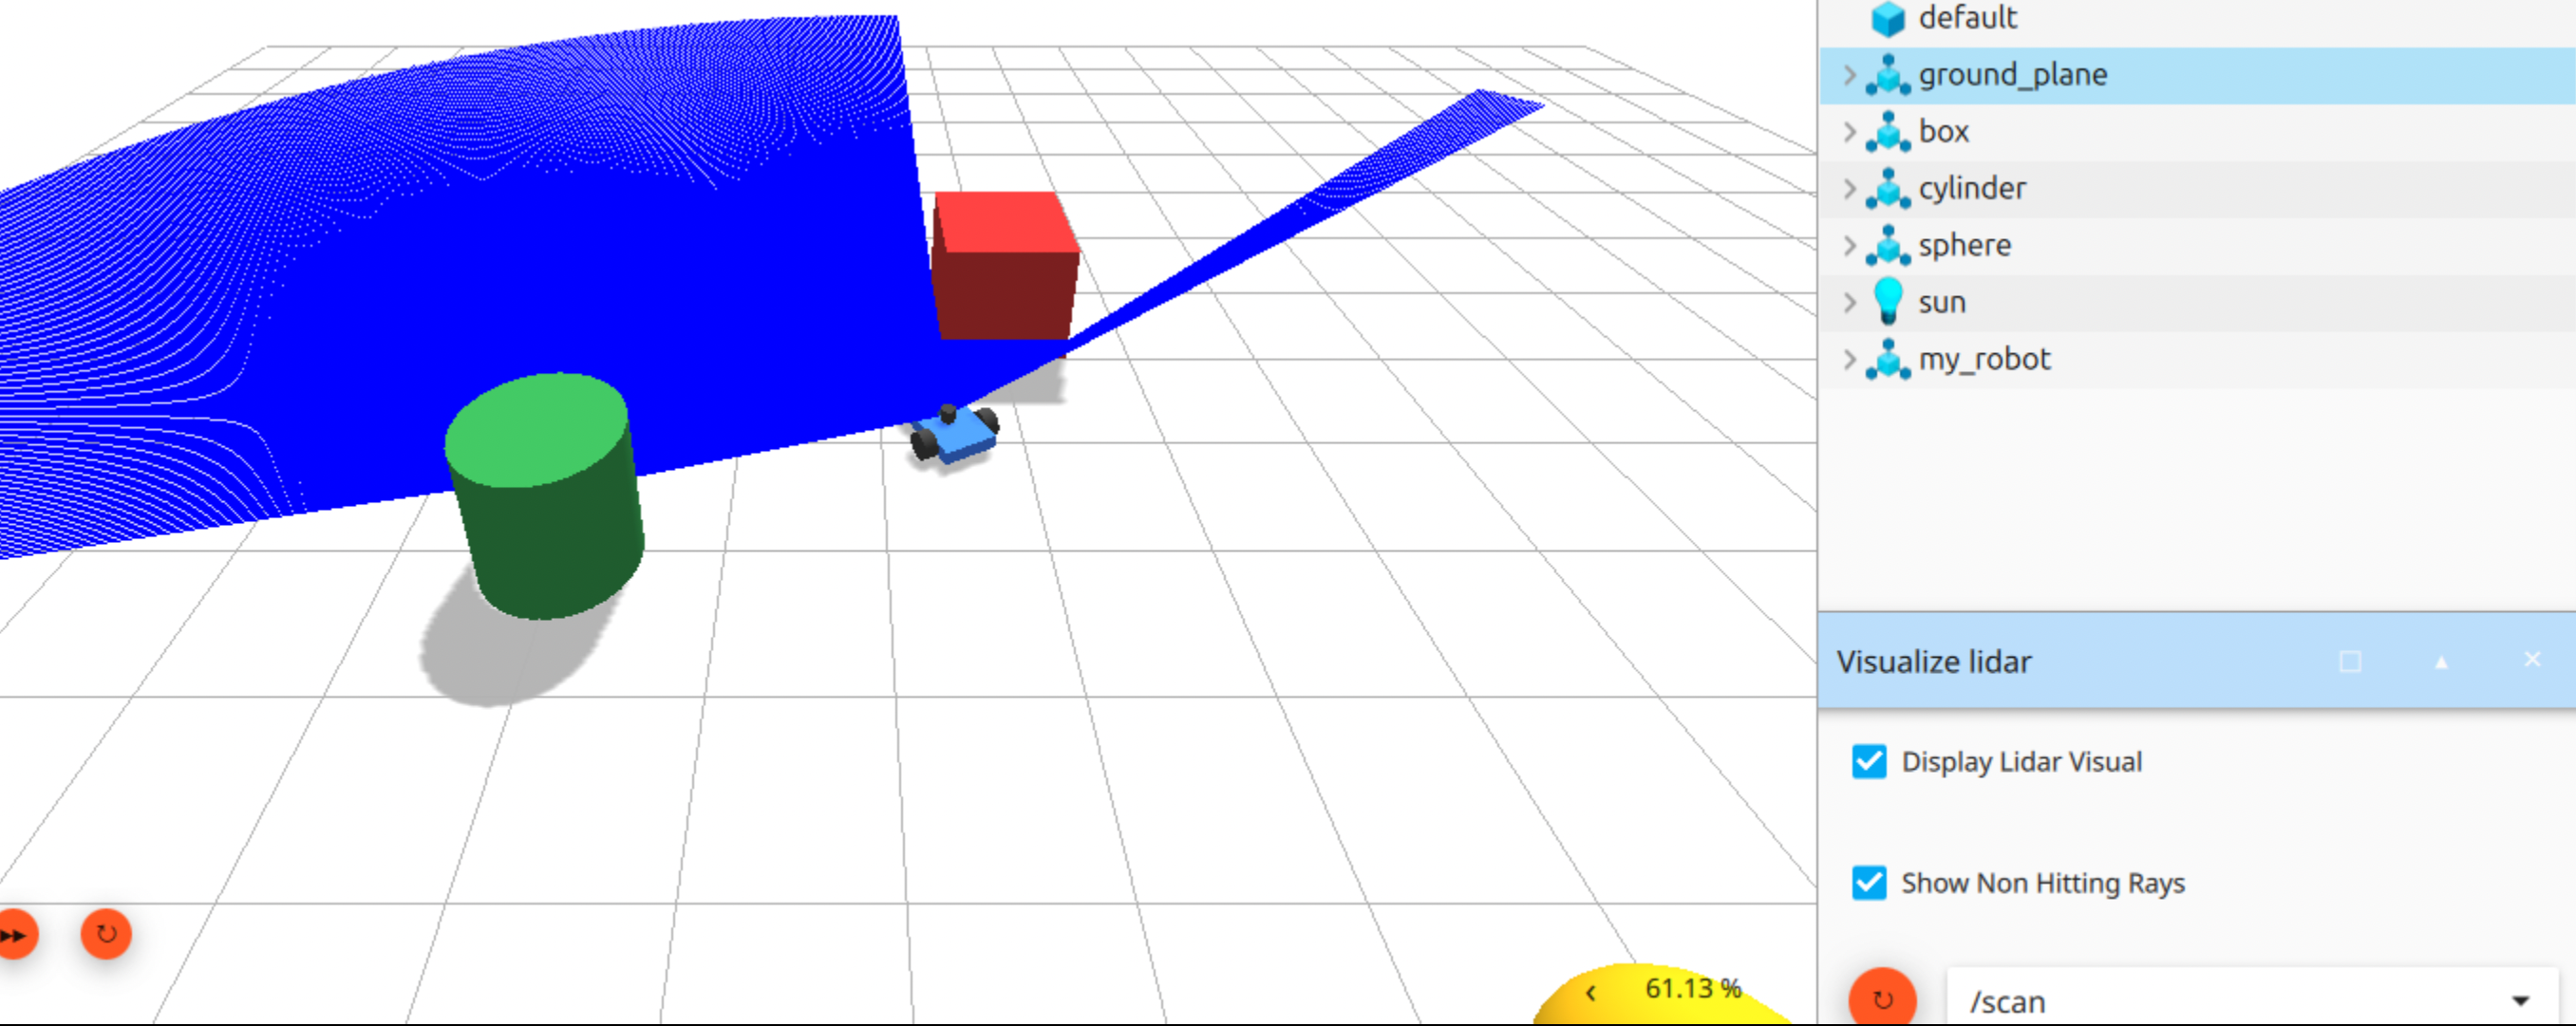
\includegraphics[width=\linewidth]{fig/Task4/03_closerScanGz.png}
        \caption{Gazebo}
    \end{subfigure}
    \\[6pt]
    \begin{subfigure}{\columnwidth}
        \centering
        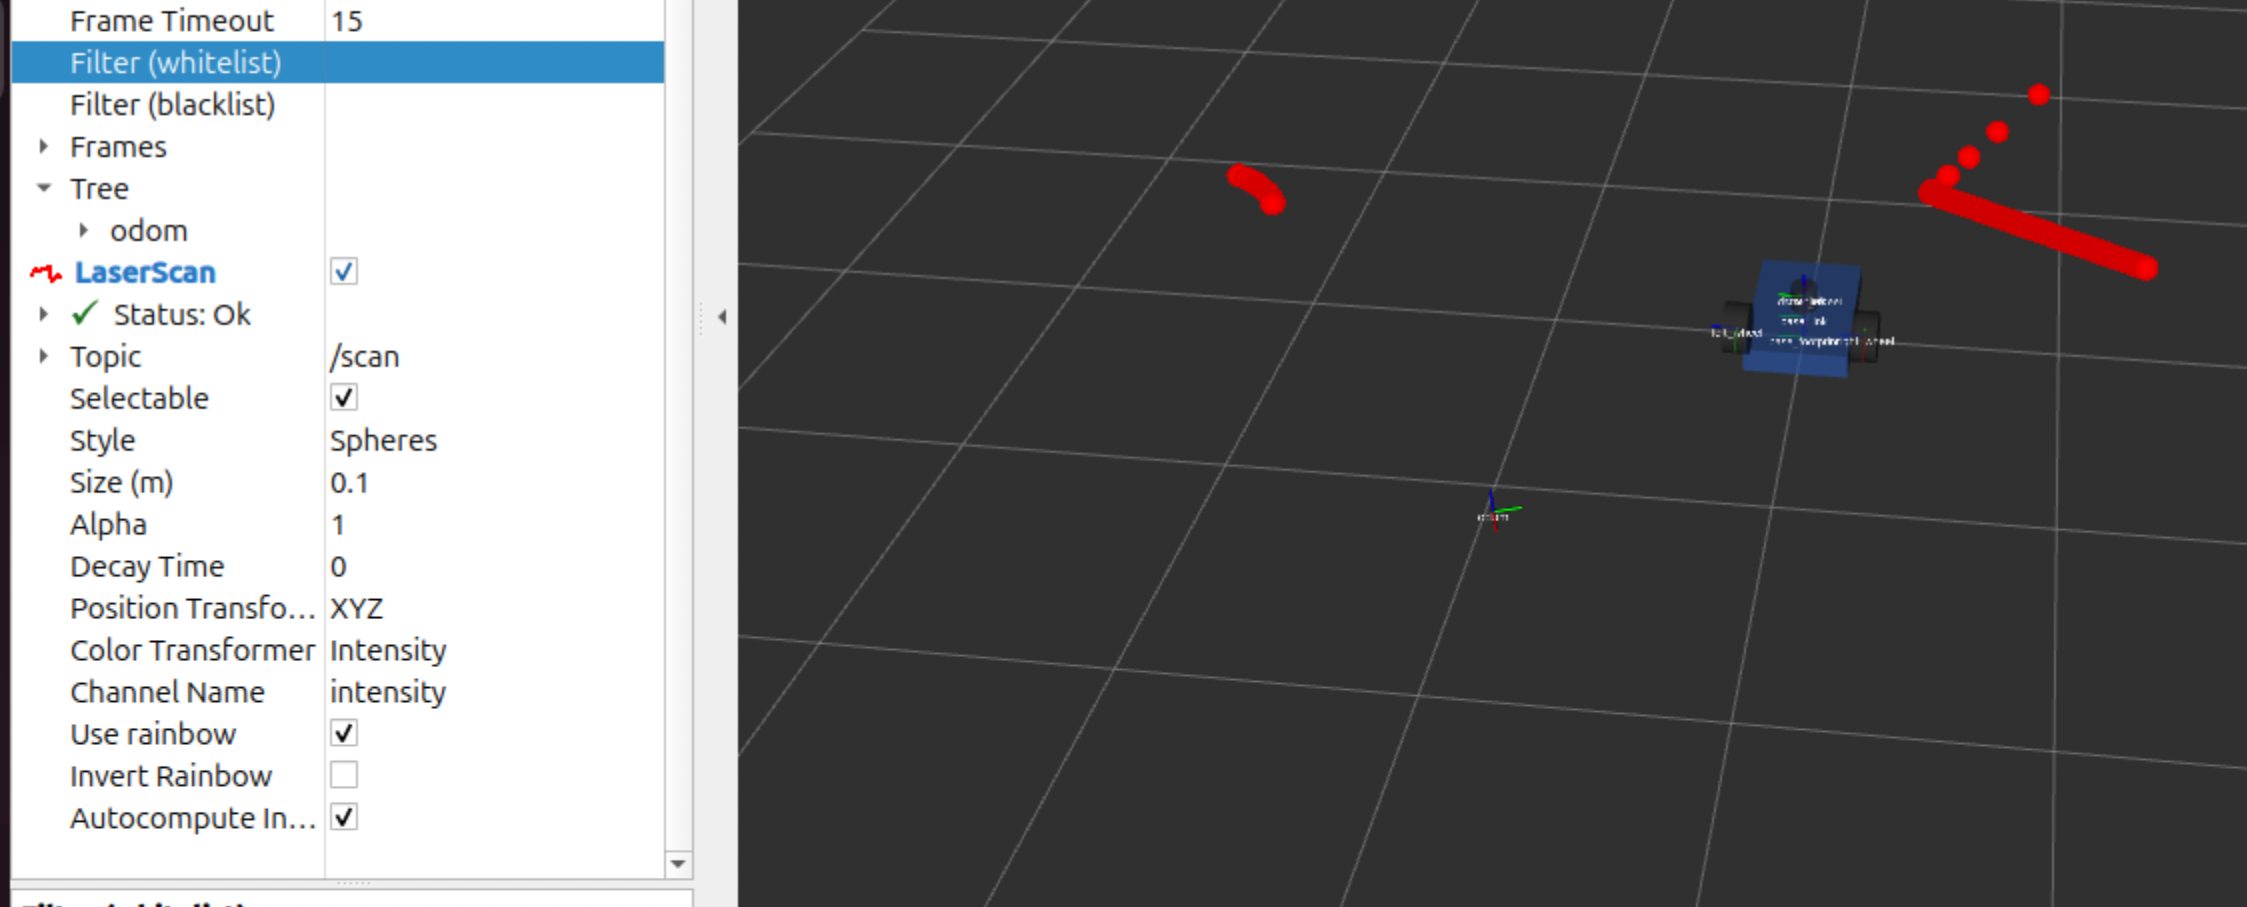
\includegraphics[width=\linewidth]{fig/Task4/02_closerScanRivs.png}
        \caption{RViz}
    \end{subfigure}
    \caption{The same scene with the robot close to the box. The returns move
             nearer to the robot and become denser, since more rays fall on the
             surface.}
    \label{fig:t4_near}
\end{figure}

\section{Reflection}
As with the last assignment, we had some frustrating fun implementing assignment 2. For task 1, we had problems with the launch file. 
We had apparently made some mistakes that made the RViz visualization of our robot show that the back wheels were gone. It turned out that we had made errors both in the macros we made and in how the launch file handled the new macros. We also split the .urdf into different files, and that caused some confusion in the beginning. We tried running xacro on parameters.xacro and my\_robot\_core.xacro, and then we got errors that told us the properties like wheel\_radius were not defined. We later discovered that this was not a bug and that properties are defined in parameters.xacro, and the other files only use them. So on their own, they don't know what the values are. We discovered that xacro reads top to bottom, so a value has to exist before it is used. This is why my\_robot.urdf.xacro includes parameters.xacro first.

For task 2, we had problems with the fact that we made the world too dark, and we tried to fix it for some time, but the visualization in Gazebo was still dark. It turned out that we still had a stalled run in the background that was overwriting the new run. We probably spent 1 hour debugging this interesting issue. We then finally checked the running process and found that four Gazebo servers were running at the same time, because it looked like Ctrl+C on the launch file did not kill the Gazebo sim process. The window we were looking at was showing a robot from a session we started 2 hours earlier. This also explained why the robot was stuck at an obstacle, and the world was using dark colors. We also had some problems with the bridge that made the visualization in RViz give us warnings. The first error we made was that we forgot to add a dash in front of each entry in the config file itself. For the keyboard integration, it took us some time to get the integration correct, as the robot would not drive. Part of this was the stale Gazebo servers, since our commands were going to one server while we were looking at another. Lastly, we tried to do the commands in the Gazebo window, but the robot did not move, as we needed to paste the commands in the running terminal. 

For task 3, we used some time to get the LiDAR Sensor correctly mounted on top of the robot according to the task description. For a while, we thought the sensor itself was broken because checking the topic showed no publisher at all, but this was the stale servers from task 2. We also experienced the VM freezing when running Gazebo. We fixed this by checking leftover simulation processes and killing them before launching again. 

Lastly, for task 4, we used some time to get the visualisation in RViz correct. We thought that we had gotten it correct but did not understand how to show it visually. After looking at the task description and screenshots attached to the assignment, we saw which setting we needed to enable. The last thing we did not do properly was that in the settings we did not set the topic to /scan. After that, the visualization finally worked. 

\end{document}
